%-----------------------
% PREAMBLE
%-----------------------
\documentclass[12pt]{report}
\usepackage[utf8]{inputenc}
\usepackage[english]{babel}
\usepackage{appendix}
\usepackage{graphicx}
\graphicspath{{figures/}}
\usepackage[a4paper,top=20mm,bottom=30mm,width=140mm]{geometry}
\usepackage{pdflscape}
\usepackage{afterpage}
\usepackage{float}
\usepackage{subcaption}
% \usepackage{subfig}
\usepackage[
    backend=biber,
    style=ieee,
    urldate =comp
  ]{biblatex}
 
 \addbibresource{references.bib}

\setcounter{tocdepth}{0}
\newcommand\tab[1][0.75cm]{\hspace*{#1}}

\newcommand\blankpage{%
    \null
    \thispagestyle{empty}%
    \addtocounter{page}{-1}%
    \newpage}

\usepackage{fancyhdr}
\pagestyle{fancy}
\fancyhead{}
\fancyhead[C]{\leftmark}
\renewcommand{\headrulewidth}{0.4pt}

\usepackage[]{algorithm2e} 
\usepackage[nottoc]{tocbibind}
\usepackage{url}
\usepackage[some]{background}
\usepackage[intoc, english]{nomencl}
\makenomenclature
% \renewcommand{\nomname}{List of Abbreviations}

% \setlength{\parindent}{4em}
% \setlength{\parskip}{1em}
% \renewcommand{\baselinestretch}{1.25}
\usepackage{setspace}

\usepackage[some]{background}

\SetBgScale{1}
\SetBgContents{\parbox{10cm}{%
      \Huge Draft:  \today\\[14cm]\rotatebox{180}{\Huge Draft:  \today}}}
      \SetBgColor{gray}
      \SetBgAngle{270}
      \SetBgOpacity{0.2}

%-----------------------
% FRONT PAGE
%-----------------------
\begin{document}
\begin{titlepage}
    \newgeometry{width=150mm,top=40mm,bottom=40mm}
    \BgThispage
    \begin{center}
        \vspace*{1cm}
        Department of Computing\\
        Goldsmiths, University of London\\

        \vspace*{3.25cm}

        \textbf{\LARGE Augmented Reality Navigation System\\}
        \vspace*{0.20cm}           
        \textbf{\LARGE for Commercial Spaces}\\
        \vspace*{0.55cm}           
        {\large Proposal}\\
        \vspace*{0.15cm}           

        \vspace*{2cm}
        by\\
        \vspace*{0.25cm}   

        \textbf{Arif Kharoti, Nicholas Orford-Williams, Hardik Ramesh,\\}
        \textbf{Gabriel Sampaio Da Silva Diogo, Hamza Sheikh, Jonathan Tang\\}
        \vspace*{0.1cm}    
        Software Projects – Group 14\\  

        \vspace{2cm}

        Autumn 2018
        \vfill

        Submitted in partial fulfillment for the degree of\\
        \textit{Bachelor of Science} in \textit{Computer Science}

        \vspace{1.5cm}

    \end{center}
\end{titlepage}

\afterpage{\blankpage}

\thispagestyle{plain}
\pagenumbering{roman}

%-----------------------
% ABSTRACT
%-----------------------

\newgeometry{top=25mm,bottom=30mm,width=140mm}
\begin{center}        
    \large
    \textbf{Abstract}\\
\end{center}

This proposal presents the use of augmented reality in museum navigation on mobile devices. After conducting stakeholder research, there were clear issues presented by current solutions on the market through the form of paper maps. AR library research was conducted on various platforms to find the appropriate one for the proposed system, and UI/UX prototyping prioritised key design aspects on the potential systems. Following this, technical architectures and user stories are defined through the MVC architectural pattern, along with technologies to be used during implementation. Methods and approaches to implementation are outlined, namely through the agile methodology along with consulting various testing methods.

\vspace*{1.5cm}
\begin{center}    
    \large
    \textbf{Word Count}\\
    xyz\\
    \normalsize computed by \texttt{TeXcount}
\end{center}

\vspace*{1.5cm}
\begin{center}    
    \large
    \textbf{Supervisor}\\
    \normalsize Dr. Basil Elmasri
\end{center}

\afterpage{\blankpage}

%-----------------------
% TOC & NOMENCLATURE
%-----------------------

\setcounter{tocdepth}{0}
\tableofcontents

\setcounter{tocdepth}{1}
\listoffigures

\nomenclature{AR}{Augmented Reality}
\nomenclature{FR}{Functional Requirement}
\nomenclature{GDPR}{General Data Protection Regulation 2016/679}
\nomenclature{GPS}{Global Positioning System}
\nomenclature{IDE}{Integrated Development Environment}
\nomenclature{IP}{Intellectual Property}
\nomenclature{MVC}{Model-View Controller}
\nomenclature{NFR}{Non-Functional Requirement}
\nomenclature{SDK}{Software Development Kit}
\nomenclature{TDD}{Test Driven Development}
\nomenclature{UI}{User Interface}
\nomenclature{UML}{Unified Modeling Language}
\nomenclature{UX}{User Experience}
\nomenclature{VR}{Virtual Reality}
\printnomenclature[1in]

\afterpage{\blankpage}

%-----------------------
% CHAPTERS
%-----------------------

\chapter{Concept Introduction \& User Needs}
\pagenumbering{arabic}
% This should explain your project idea. You can presume that the reader has a basic level of technical knowledge but not specific knowledge of your particular area, so communicate your ideas clearly.

The main concept for this project revolves around the use of augmented reality (AR) navigation on smartphones. AR is the superimposing of a computer-generated image onto a user's view of the real world \cite{oxforddict}. This technology first came about in the 1960s \cite{InteractionDesign} but has recently gained wide-spread consumer and media attention after the use of on Snapchat filters \cite{Snapchat} and the 2016 game \textit{Pokémon Go} for example. There have been many times where people get lost in unfamiliar spaces such as a museum, immersed by the culture around them, and their sense of direction. This project aims to tackle this issue by allowing users to restore their orientation by having a mobile platform to route users to their destination, using AR. The platform will use the device's camera to work out its surrounding, and will produce a highlighted line on the screen to their destination in real time.\\

This concept has various applications to other similar scenarios such as finding products in a supermarket, books in a library, or even valuable items that people own that can emit an electronic signal for it to be tracked down. Further, the concept could also use machine learning in identifying user's traits in places visited in a museum in order to give personalised recommendations at other similar exhibitions.




\chapter{Stakeholder Requirements}
% You should identify the stakeholders of any software you are developing and reason that they have an interest in your concept.

After consulting with the main stakeholders are museum visitors and staff, and potential users of the proposed application, a better understanding was available, concerning the apparent need that was in the relative market regarding museums. Out of the 21 responses received, 15 potential users admitted to visiting museums at least once a month; showing some level of frequency in their visits, and that something can be offered to this group of people.\\

Since the concept principally considers the use of navigation in museums, when users were asked, "do you find yourself using the maps in the museum more than once?"- 100\% of visitors agreed that they referred to the maps around the museum multiple times, and some respondents over 10 times. However, these maps are not free; in most museums, including the Natural History Museum and the Science Museum in London, require a fee of £1.\\

18 of the respondents agreed they preferred using their phone to navigate rather than the paper maps. Outlining a clear need for an accessible tool other than the maps around the museum.\\

Based on the stakeholder research, the project requirements are, 

\begin{itemize}
    \item navigate the user to a museum through the use of augmented reality
    \item to display navigational routes in real time
    \item calculate the shortest route to the user specified location 
    \item work transferrably in other museums/commercial spaces
    \item contain accessibility features such as magnified text and inverted colours for example
\end{itemize}

Another key stakeholder are museum staff as they are instrumental to any on-the-ground assistance in terms of navigation. Furthermore, the application should endeavour to make it easier for museum staff to assist visitors.\\

The stakeholder requirements of museum staff are,

\begin{itemize}
    \item Exhibit an effective and easy-to-use design. 
    \item Be economic and effective in its use of data, as most data would be sourced from the museum Wi-Fi. 
    \item Written content and other media to be within control of the museum.
\end{itemize}

During the field research, museum-floor staff and receptionists were also consulted. The staff approached had all received a navigational inquiry, either from themselves or visitors. Although positive responses were received several concerns were cited,\\

\begin{itemize}
    \item Battery performance
    \item Data usage
    \item Ease of use
\end{itemize}


\chapter{Prior Knowledge}
% You should describe how you gathered relevant information for credible sources, summarised and analysed that data, and how that information altered the proposed concept. 
% Computer Science: you should explain the computer science problems presented by your project, satisfying the programme learning outcome “Apply computational thinking to the design and implementation of moderately complex computing systems”.

\section{Current Solutions \& Competitors}
The market of indoor museum navigation has grown recently with more solutions being submitted due to the growth in indoor navigational research. Most solutions cater well for a basic navigation of large public spaces, but fail to display an even proportion of navigational, and interactive content with well-presented data.\\

Since most museums use portable audio guides, user experiences can be vastly improved by mobile devices. Currently only a few solutions can be found; the Orpheo group \cite{orpheo} provide a unique app for each place; their solution is cumbersome to regular museumgoers who wish to have a hassle-free setup. As the aim is to appeal to museums, having an application whereby the user can walk into a museum, and greeted with relevant information is vital in comparison \cite{microsoft}.\\

If museums wanted a solution for navigation, due to the low number of museum-specific competitors, would choose to use a standard indoor mapping software \cite{engadget}. However, while there are many options out there from Google and Mapspeople \cite{mapspeople} who try to provide this, they lack exigencies that are imperative for museums like heavily-integrated AR, and intelligent tour guiding from your location.\\ 
% and virtual reality to take a scene from the museum, for instance, and place the user to the artefact's original time and place.\\

From a technological viewpoint, a problem in the solutions that museums implement today, would be their paper maps not processing real-time locations. AR allows for real-time data processing, picking up the user's current location, and displaying the best route for the user to take through their device's camera. A benefit of implementing AR is the unique approach to today's navigation solutions, whilst allowing users to create their own content, enabling more opportunities to interact with the application.


\chapter{Design}
\documentclass{article}
\usepackage[utf8]{inputenc}
\usepackage{graphicx}
\usepackage{float}

\author{Hamza Sheikh}

\begin{document}

\subsection{The Importance of Design}

Design is a great initial investment owing to a number of different reasons. Having a design process allows for more efficiency and transparency when actually coming to design the application. It overcomes the risk of having to refer back to the drawing board when actually developing the application, setting in stone the main features and functionality of the application.\\

\subsection{The Unified Modeling Language}

A way in which effective design strategies were carried out was through the implementation of the Unified Modeling Language (UML), a powerful standard for creating specifications of various parts of a software system.\\

\\One example of the UML was our implementation of a use case diagram which outlined the different scenarios in which a user would function the application. See figure~\ref{fig:Use Case Diagram}.\\

\begin{figure}[H]
    \centering
    \includegraphics[width=\textwidth]{use_case.pdf}
    \caption{Use Case Diagram}
    \label{fig:Use Case Diagram}
\end{figure}

\\Another way in which UML was implemented to further support and refine the designing phase of the software development was through an activity diagram. (See figure~\ref{fig:Activity Diagram}).

\begin{figure}[H]
    \centering
    \includegraphics[width=\textwidth]{Activity_Diagram.pdf}
    \caption{Activity Diagram}
    \label{fig:Activity Diagram}
\end{figure}

\\The use case diagram (Figure~\ref{fig:Use Case Diagram}) represents the functional behaviour of the system in terms of goals that can be fulfilled by the system. These goals have been defined in the stakeholder requirements. The activity diagram (Figure~\ref{fig:Activity Diagram}) was designed to model the work flow of the system. One main reason that the activity diagram was essential in the designing phase was that UML included that these diagrams are normally easily comprehensible for both analysts and stakeholders. By producing and creating these models, we were able to have a clear understanding of what the application \textit{has} to do, and enabled us, the developers, to visualise the application for the future.

\subsection{Service Model}

We have to first exclaim that the following cases are born out of one important principle; convenience. The \textbf{'lost'} use case, for example, comes from the fact that the user could be lost for whatever reason. What we would provide through this service would be the quickest and most \textbf{convenient} solution to finding their destination. Whether that be the exit, a cafe or a particular exhibition. Another use case;
\textbf{'exploration'}, would become more convenient with the museum, and all its exhibitions (along with brief descriptions) at your fingertips (instead of the existing navigation options present at museums today e.g. wall-maps or paper maps).
\subsubsection*{Model around two cases (The lost and the exploring) }
The lost-case and exploration-case has a virtually linear-stream of logic, and is as follows:
\begin{enumerate}
    \item The user enters within the radius of an environment modelled by the service. In this case, a museum.
    \item The user’s location is picked up once they give use permission to (in this case, it would typically be when the user opens the app). 
    \item The user then picks their destination.
    \item That location is then taken and parsed through a function containing an algorithm that calculates the most convenient route between the user’s real-time location and their desired destination.
    \item The user is then displayed the route, and directed towards their destination via their camera.
    \item Once done, the user is given curated suggestions on possible places they can go.
\end{enumerate}

\end{document}



\chapter{Prototyping}
% Describe the prototyping you did, and what you learned from this, particularly the low fidelity interaction prototypes, any technical prototypes to explore technical feasibility of the solution, and the functional digital prototypes that you used with users to validate that what you are developing meets the expectations of users.

\section{Augmented Reality Libraries}
In order to identify libraries that are good for implementing AR on mobile devices, we divided this prototyping into three platforms to explore them, and built test applications to find out how they help with the project.

\subsection*{Vulforia (Unity/Android)}
Unity is a cross-platform game engine, used to test a simple AR camera prototype where the device's camera hovers an object/image, and displaying information about that object/image on the device. The application was built using Vuforia, an SDK that enables recognition, and tracking of image targets. This library can be used for the exploration case in the use case model. Although, there is a limited amount of tools for locating user current location compared to Android.

\subsection*{ARKit (iOS)}
A similar prototype to Unity was built on Apple's ARKit using Swift \cite{applear}, which was easy to learn. It was intuitive to implement AR features as there was detailed documentation but logging GPS data was harder compared to Android.

\subsection*{ARCore (Android)}
ARCore was used to create a simple 3D model showing on a mobile device when its camera targets a flat surface. Compared to iOS, it is easier to log GPS location, although connecting the user interface to the scripts was more challenging.

\section{User Interface/User Experience Designs}
The project lends substantial importance to its user interface and experience. As it will be used from a wide cross section of technical ability, the aim for UI will be to make the app as simple, and easy to use as possible without having an impinging effect on any major service the end product will feature. This prerequisite was clearly outlined in the surveying of museum guests and staff alike. Our first mission was to determine what interfaces, and experiences current exists within the museum sector. Many museums did employ simple interfaces but due to their mass-manufacturing, their design felt unoptimized, slow and clunky, with simple barebones media not beyond text and images. Furthermore, this design would fail to deliver anything more complex than texts and images.\\
  
The approach to the UX/UI prototyping was to create a score of different complete interface mockups and exhibit them alongside existing solutions. Three team members independently drew up potential interfaces. These candidates were then put to stakeholders, and all received positive attributes were combined into one.


\chapter{Functional Specification}
% The essential functional elements should be defined and described, including data paths. This functional specification should not assume any specific technologies, only functional technologies (e.g. short range wireless technology is a functional statement whilst Bluetooth is a specific technology)

The main functional elements of our concept are:

\begin{enumerate}
\subsection*{Route Calculation}
    \item Receiving the \textbf{current coordinates} of the user, and the coordinates of the destination will be needed to create the starting and end points for calculating the route. The current location will come from sensors on the user's device, and the destination location will be queried against a mapping system.
    \item The platform can \textbf{calculate the quickest route between two points} specified by the user. Data from the above, and the museum model will be required for this calculation.
% \end{enumerate}

\subsection*{Superimposition}
% \begin{enumerate}
    \item A \textbf{3D line will be superimposed} that navigates the user to their destination. Sensor data from the user's device along with the user's relative position in the model will be required to show the line. Access to the user's camera is essential in this element.
% \end{enumerate}

\subsection*{Suggestion/Reviewal}
% \begin{enumerate}
    \item When the user arrives at their destination, the \textbf{system will give recommendations} based on their current route, and allow the user to rate their journey.
    \item The \textbf{user's camera can recognise artwork/objects}, and will display further information about the piece. There will be a storage area of current pieces in the museum so that the camera can query the information.
\end{enumerate}



\chapter{Technical Architecture}
% Having validated the proposed solution with users and answered any open technical or feasibility questions, attribute specific technologies to the functional architecture and present this as a technical architecture. Justify your choice of technologies with reasoned arguments for rejecting or retaining alterative technologies.

\section{Means of Software Development}

\subsection*{SDKs}
Google's \textbf{ARCore} kit gives us the ability to apply the AR element of the application without having to spend time pre-defining AR methods. It has distinct advantages over Apple's ARKit as ARCore can detect horizontal surfaces that is similar to motion tracking, and can accurately anchor virtual objects. \cite{newgenapps}

\subsection*{Platform \& Languages}
The app will be developed on Android since ARCore only works on that platform. Java is imperative to the project since android development is only possible in this language.

\subsection*{IDE}
\underline{Android Studio} is the IDE utilised in the project because it involves a number of relevant exclusive packages. Other IDEs, requires them to be pre-defined, and therefore takes out valuable time from application development.

\subsection*{Architectural Pattern}
Our application fits under the MVC pattern perfectly be it that the following are true.
\begin{itemize}
    \item Model: Data provided by the user (e.g. geolocational data)
    \item View: Front-end interface (e.g. 3D line to location)
    \item Controller: Algorithms between the model \& view (e.g. route calculation)
\end{itemize}
The pattern's simplicity makes the most sensible one we can use.

\newpage

\section{Satisfying user-related questions from the user stories}
\subsection*{Questions}
\begin{enumerate}
    \item How will the navigation system get me from point A to point B? (Figure~\ref{fig:AtoB})\\\\
    In order for user to get from one point to another, it will use route calculation to calculate the quickest route.\\
    Route Calculations:
    \begin{itemize}
        \item Algorithms to request and process GPS signal.
        \item Algorithms to calculation quickest route when user enter their destination.
        \item Once calculated, show the result for user to start their journey.
    \end{itemize}
    
    \item How easy will it be to grasp the app?\\\\
    The layout would be simple and the basic map/guidance will work straightforwardly. Once the route has been calculated, a 3D line will be superimposed on the users screen.
    
    % \item When I open the app, what will I see? \\\\
    % When user opens the application, the first thing they will see is the main page. For example, sign in/guest users, and service utilities.
    
    \item Can the app be used without Internet? \\\\
    No, otherwise the app would not have access to the user's real time location, and would take up too much storage space on the user's device if it was used without.
\end{enumerate}

% \subsection*{User Stories}
% % There are three crucial user stories - they're shown below.
% The user stories satisfies our architectural pattern and can be easily realised with our technical infrastructure. \textbf{ARCore} and functions provided by \textbf{Android Studio} provide us with predefined technicalities such as superimposition, and real-time geo-spatial data which allow us to lay the foundations of all three processes.


\chapter{System Requirements Specification}
%This bring summarise and bring together all the previous section into a specification that should be fully expanded in the appendix with the following points, in providing what is known as the System Requirements Specification (SRS). This collects various information that you have previously agreed and worked on such as the UML diagrams.

% SRS contents:
% 1. Purpose
% 2. Scope
% 3. System Overview
% 4. References
% 5. Definitions
% 6. Use Cases
% 7. Functional requirements
% 8. Non-functional requirements.

\section{Difference between functional requirements (FR) and non-functional requirements (NFR)}\\

The nature of the application is a tool used to support navigation around musuems, through the implementation of AR. There are two main types of requirements that the Systems Requirements Specification comprises: Functional and Non-Functional requirements. The functional requirements specify \textit{what} the system should do. Whereas, the non-functional requirements specify \textit{how} the system should perform a function.\\

One example of how these requirements would differ would be that, the system being able to successfully calculate the best route to their desired destination would be a functional requirement as it is something that the application is set out to provide for the user. However, the graphical interface and the design of the application may not be a functional requirement as it is not an aspect of the system that is required to solve the user's problem.

%\subsection{What are functional requirements?}
%A requirement that describes what the system should do. In other word, it should express the behaviours of function of the system when certain conditions are made for example making an AR system to help navigate around the exhibit.

%\subsection{What are non-functional requirements?}
%It's a requirement that described how the system should perform a certain function. It will describe the behaviour of the system and limits.

\subsection{Difference between FR and NFR}
The functional requirements are the most critical then FR because even if we missed one or two FR, the system will work properly whereas if we missed any NFR their will be problem where system can became useless. This is why we need to focus more on NFR.
\begin{enumerate}
    \item Functional requirement include in our project:
    \begin{enumerate}
        \item Needs to be able to navigate the user from point A to B.
        \item The app should be able to display navigational routes in real time.
        \item It should be able to calculate the quickest route.
        \item A 3D line will be superimposed that navigates the user to their destination
        \item The user’s camera can recognise artwork/objects, displaying further information about the piece.
        \item when user arrives to their destination, the app will give recommendation based on their current route.
    \end{enumerate}
    \item Non-functional requirement include in our project:
    \begin{enumerate}
        \item Performance -  The app should have quick response whenever a user wants to find more information about an art piece or whenever they search up a location. As well as that, it should not slow down their phone to avoid negative impacts.
        \item Usability - The app would be layout simple, there would be some colours used for appropriate purpose. The language used on the app would be easy to understand for the users. Having done research based on the user preference, it was discover that users tend to dislike having too much displayed on their menu screen all out once. Therefore, the app would take the user step by step to make it more user friendly.
        \item Data Usage - the app would need internet connection in order for it to work out the real time distance and the length of the final destination.
    \end{enumerate}
\end{enumerate}




\chapter{Ethical Audit}
% You should detail any issues of privacy, data protection or intellectual property rights that may arise, and how you will manage them. You should confirm that you will not be working with minors or vulnerable adults.

AR is currently not heavily regulated in the UK owing to the emergence of this new technology. It should be noted that AR will involve collecting extensive amounts of data per user such as names and emails, but also real-time location, and interactions with other users. Within the scope of this project, we will not be working with minors and vulnerable adults. Since the project concept relies on the user's camera, accelerometer, and GPS on the user's device, ensuring this data cannot be obtained unlawfully, fitting the scope of the Data Protection Act (1998), and GDPR is of most importance.\cite{ITProPortal}\\

Based on large VR companies such as Oculus, these obligations are addressed by a privacy policy, to detail how data is collected, used and if it is shared with third parties. It is critical these regulatory issues are addressed before the completion of the product and not after.\\

Another regulatory standard is the IP of the software. The source code that serves as the underlying foundation of the platform will be be original and qualify for copyright protection. Since computer software is usually excluded from patentability in the UK, ideas that uses AR producing a technical effect, and its associated hardware can be protected by patents. Based on our competitors, it is important that we do not infringe on their patents owned by third parties.\\

Equally, if the concept makes new technical developments in the AR field, there should be consideration whether it would be eligible for patent protection. The project could use machine learning by recognising artworks captured on the user's camera. This could cause an infringement claim since AR could be replicating, replacing trademark or copyright works, or distorting the artwork.


\chapter{Evaluation Plan}
% How you intend to test and evaluate your software during and after development. It may be useful to specify individual test cases.
% TDD

\section*{Test Driven Development (TDD)}

TDD will be the main testing process both during, and after creation because of the following. 

\subsection*{1. Tangible results reviewed with efficacy}
As a test based method, it allows the ability to adapt, and prove what works. For example, the application requires a guiding graphic. TDD makes it easy to review whether a 3D line, is the best case solution. Or whether an alternative, such as an arrow, is better.

\subsection*{2. Simplicity of implementation}
The application as a concept, is straightforward, but is relatively difficult to manifest because of the technical complexities. To have a simple way to evaluate the application makes it easier to create. TDD can assist with the complexities of the route calculations. For example, when choosing the best route. Does the algorithm place more weight on scalar distance? Or on obstacles? TDD makes the process of making this decision distinct.

\subsection*{3. Re-usability}
The ability to iterate over multiple prototypes and algorithms with TDD makes the process of fulfilling those few purposes simpler. It also means they can be achieved with a high degree of quality.


\chapter{Project Management}
% How you will manage the development process: milestones, Gantt charts, roles, development methodology etc.
% JT will write this

During the development process we will employ the agile methodology to manage.


\chapter{Conclusion}
% Summarise your proposal, including the key points from the previous sections.

The concept is to build a solution to indoor museum navigation in the sector. The problems became clear through market research, which defined the user requirements. Upon discovering the inadequacies of current solutions; chiefly failing in succinct user navigation with museum exhibitions; instead of 2-D mapping, through the implementation of augmented reality, the project will be able to offer real-time 3-D mapping.

UML models were drawn up using stakeholder requirements to define user and activity behaviours. Research was conducted around AR libraries to find the appropriate packages for the project. ARCore stood out as it can accurately anchor virtual objects better than Vulforia and ARKit. A storyboard and three UI/UX prototypes were constructed to show stakeholders samples of the platform, combining all effective features into one. This provided an understanding of user behaviour concomitant with usability.  

From prototyping, the main functional elements were outlined. It was decided the platform will adopt the MVC architecture to aid modelling, and questions from the user stories were addressed. System requirements specification was composed to summarise, outlining features and behaviour of the system. During the system life-cycle, TDD will be used to test system components.  

Ethical auditing helped to adhere to regulations, and standards in software development. Due to the wide scope of the project, Agile methodology will be used, allowing for ease of innovation in relation to features.


\afterpage{\blankpage}
%-----------------------
% APPENDICES
%-----------------------

\begin{appendices}

\chapter{Systems Requirements Specification}
% This bring summarise and bring together all the previous section into a specification that should be fully expanded in the appendix with the following points, in providing what is known as the System Requirements Specification (SRS). This collects various information that you have previously agreed and worked on such as the UML diagrams.

\section{Purpose}
The main goal of this concept is to provide an exciting, and enjoyable experience for museum-goers through the use of AR. It includes users being lost, or searching for a specific location within the museum. The target audience is aware of this concept during the field research, it was discovered that the concept would make life easier for users and the museums since it would allow easy access to the information based on exhibitions.

\section{Scope}
This project will include creating an AR application for people to get an enjoyable journey in the museum. The project will be completed by 29 April 2019. The AR application will include simple navigation system to direct various part of the museum. Getting information on the user screen using the user's camera, and explore various museum using the app. 

\section{System Overview}
The application will perform all the basic tasks to help users with their journey in the museum. Such as navigating from point A to B, getting the user back on track in case they are lost, allowing the user to view information based on camera recognition of an exhibit.

\newpage
\section{References}
This specification should be used in conjunction with the following publications:\\
IEEE Std 610.12-1990, IEEE Standard Glossary of Software Engineering Terminology \cite{IEEE610}\\
ISO/IEC/IEEE Std 29148-2011, ISO/IEC/IEEE International Standard - Systems and software engineering -- Life cycle processes --Requirements engineering \cite{IEEE29148} \\
IEEE 730-2014, IEEE Standard for Software Quality Assurance Processes \cite{IEEE730} \\
IEEE Std 1220-2005, IEEE Standard for Application and Management of the Systems Engineering Process. \cite{IEEE1220}

% https://reqtest.com/requirements-blog/understanding-the-difference-between-functional-and-non-functional-requirements/
% https://www.tutorialspoint.com/operating_system/os_overview.htm

\section{Definitions}
\textbf{Augment reality:} AR, the main goal of this project and what makes it standout from other apps, such as Google maps.\newline \\
\textbf{User:} The person who would be using the app. \newline \\
\textbf{Route calculation:} Back-end prototype, using real time location of a user. \newline \\

\section{Use Cases}
The use cases have been defined as follows:
\begin{enumerate}
    \item Use Case Model
    \item Activity Model
    \item User \& Acceptance Stories
    \begin{enumerate}
        \item In Exhibit going from A to B
        \item Getting information from an exhibition
        \item Exploring the museum
        \item User get lost in the museum
    \end{enumerate}
\end{enumerate}

\newpage
\subsection{Use Case Model}
Two scenarios have been taken into account, where the user gets lost in the museum, and the user wants to explore the museum. When a user is lost, they need to enter their destination where the app will calculate their current location, and find the quickest route from the user's current position. The user follows that navigation until they arrive at their destination. For the exploration, the app will show the details where user know what they going to see in the museum.

\begin{figure}[H]
    \centering
    \includegraphics[width=\textwidth]
    {uml/use_case.pdf}
    \caption{Use Case Diagram}
    \label{fig:Use Case Diagram}
\end{figure}

\subsection{Activity Model}
This is based on the back-end of the application for example when the user searches about the museum, this history saved in the server where if the user wants to go to the same place then they can use our function called past visit.

\newpage
\begin{figure}[H]
    \centering
    \includegraphics[angle=90, width=\textwidth]
    {uml/Activity_Diagram.pdf}
    \caption{Activity Model Diagram}
    \label{fig:Activity Model Diagram}
\end{figure}

\newpage
\subsection{User \& Acceptance Stories}
This will describe what will be achieved once the application is ready to be used by the user. A diagram has been created based on different scenarios where it can be found if the application has achieved the user needs. 

\begin{figure}[H]
    \centering
    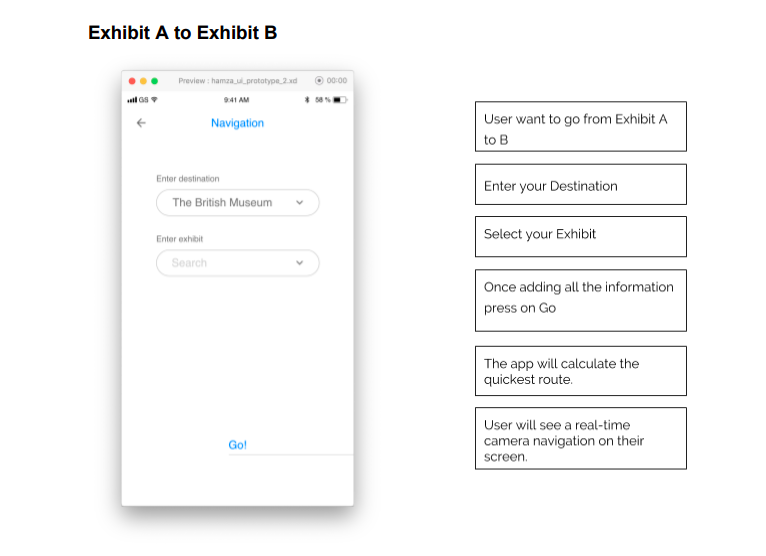
\includegraphics[width=\textwidth]
    {userstories/userstory_aTob.png}
    \caption{Going from point A to point B}
    \label{fig:AtoB}
\end{figure}

\begin{figure}[H]
    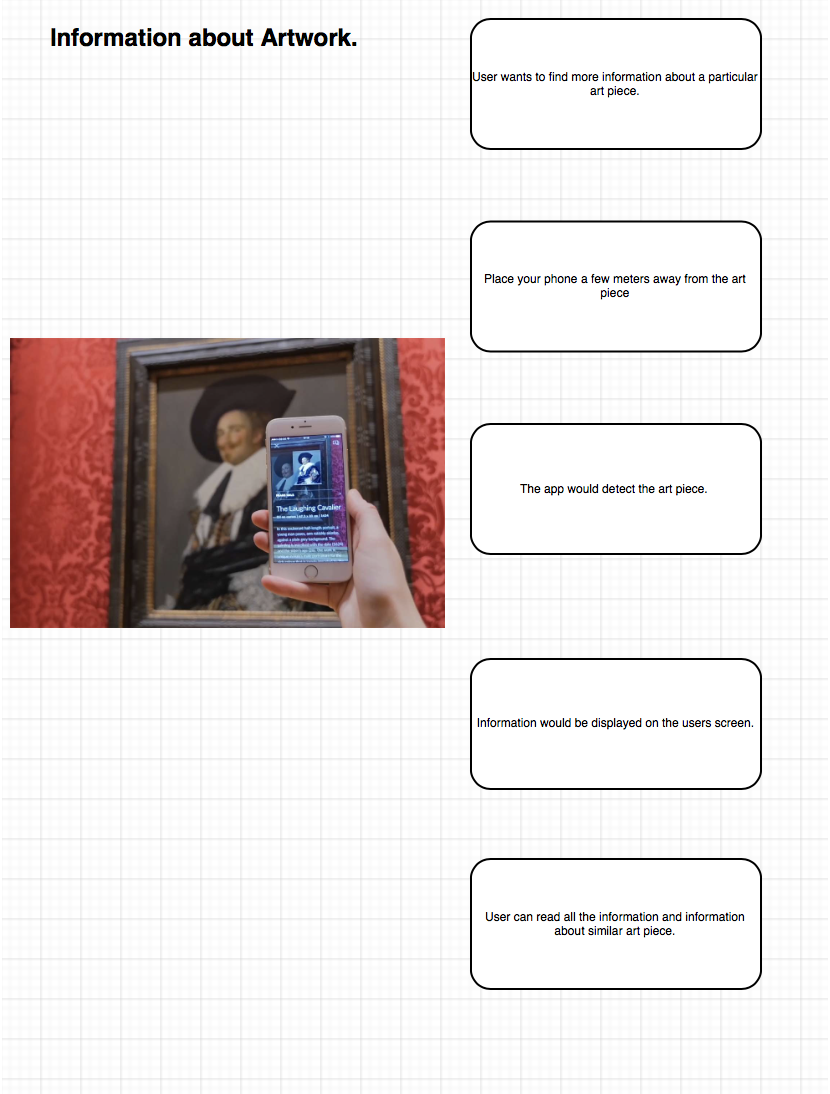
\includegraphics[width=\textwidth]
    {userstories/userstory_info.png}
    \caption{Getting information from exhibition}
    \label{fig:infofromexhibit}
\end{figure}

\begin{figure}[H]
    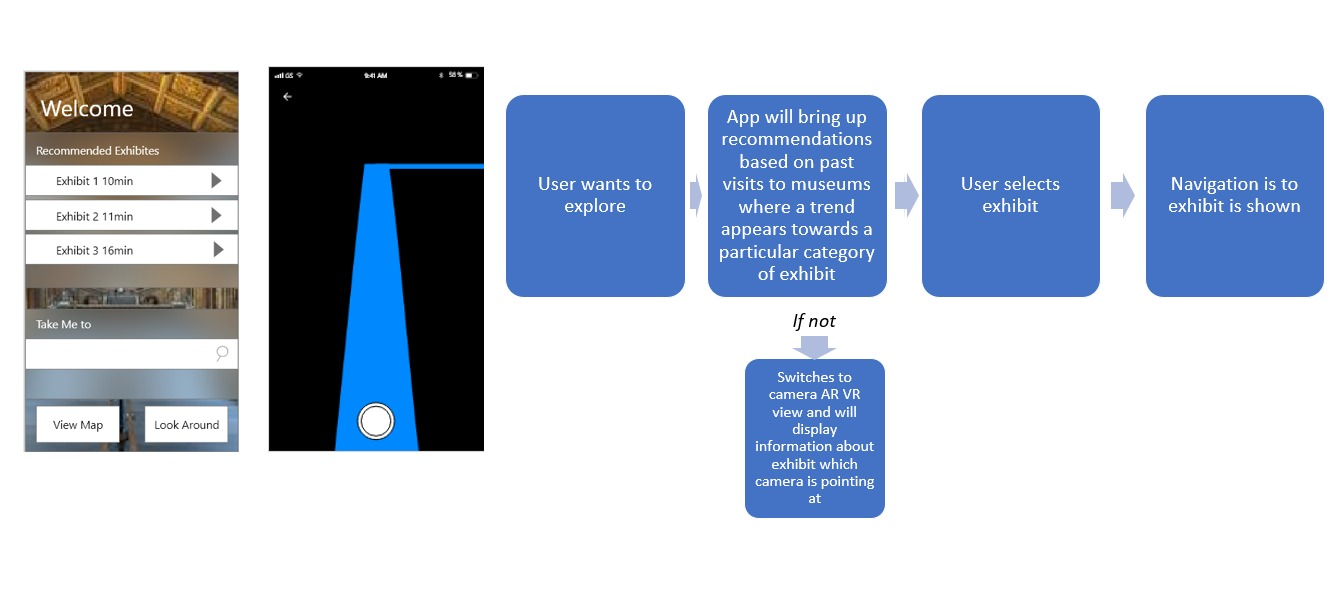
\includegraphics[width=\textwidth]
    {userstories/userstory_explore.jpeg}
    \caption{Exploring the museum}
    \label{fig:exploring}
\end{figure}

\section{Functional requirements}
\begin{itemize}
        \item Needs to be able to navigate the user to an exhibit through the use of AR.
        \item The app should be able to display navigational routes in real time.
        \item It should be able to calculate the quickest route to a destination.
        % \item Should be able to work in other museums
\end{itemize}

\section{Non-functional requirements}
\begin{itemize}
        %\item Security is one of the most important parts of this project because the application stores username/passwords. The application will use MySQL to store data in the database and this will help to secure user data in the system.
        \item Performance -  The app should have quick response whenever a user wants to find more information about an art piece or whenever they search up a location. As well as that, it should not slow down their phone to avoid negavtive impacts.
        \item Usability - The app would be layout simple, there would be some colours used for approraite purpose. The language used on the app would be easy to understand for the users. Having done research based on the user perfences, it was discorved that users tend to dislike having too much displayed on their menu screen all out once. Therefore, the app would take the user step by step to make it more user friendly.
        \item Test driven development - 
        \item Data Usage - the app would need internet connection in order for it to work out the real time distance and the length of the final destination.
\end{itemize}
    



\chapter{Figures}
% The appendix or appendices should contain your group meeting minutes and any additional raw material that is referred to in the text (e.g. data from requirements gathering, paper prototypes etc.)
\section{Prototyping}
\subsection{AR Prototypes}
\subsubsection{Vulforia}
\begin{figure}[H]
\centering  
\begin{tabular}{cc}
  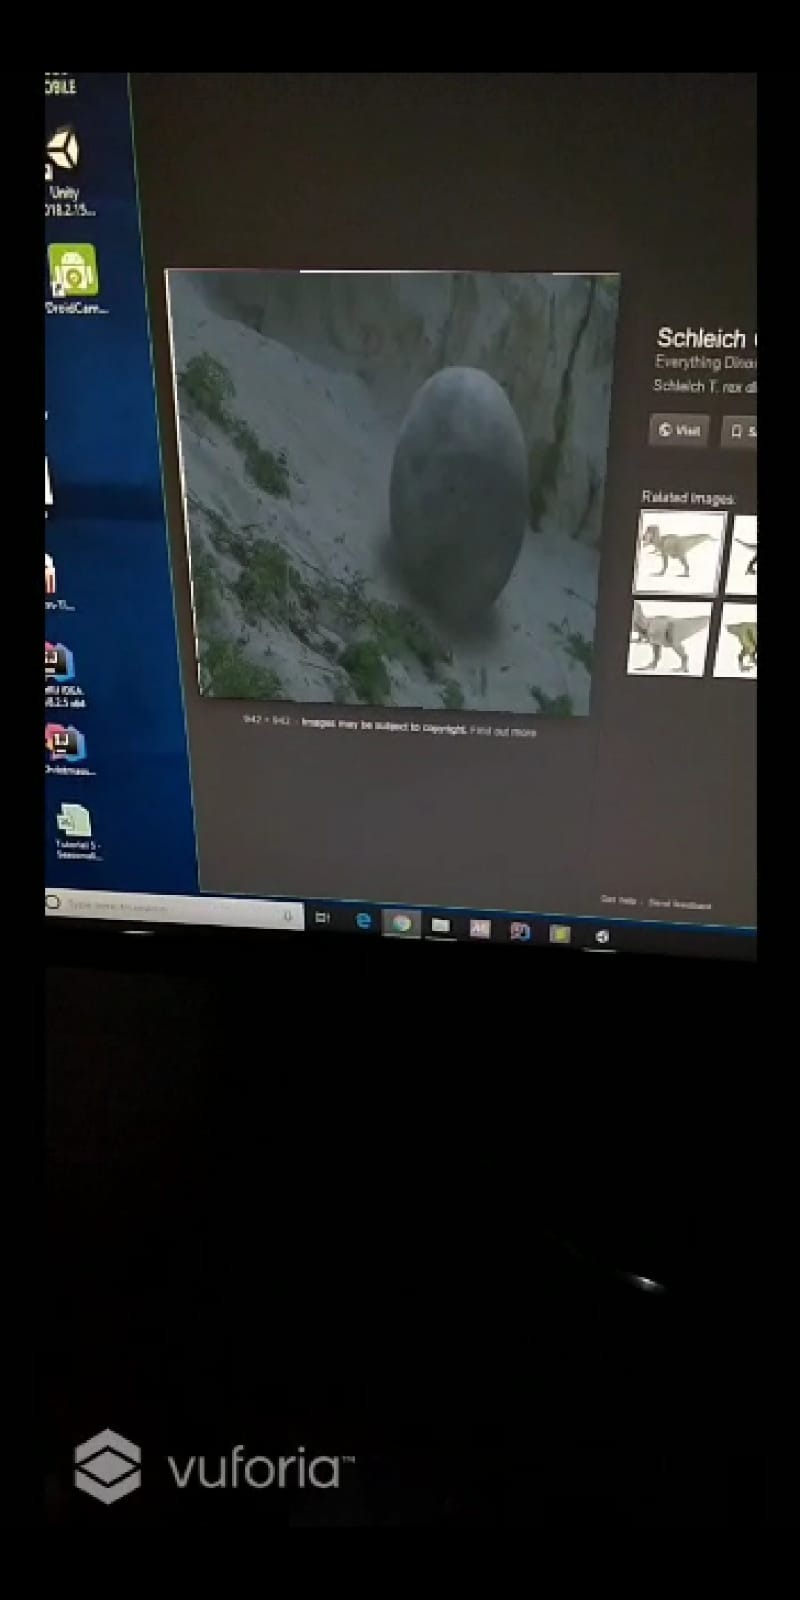
\includegraphics[width=60mm, height=100mm]{prototypes/ar/vulforia/1.jpeg} &   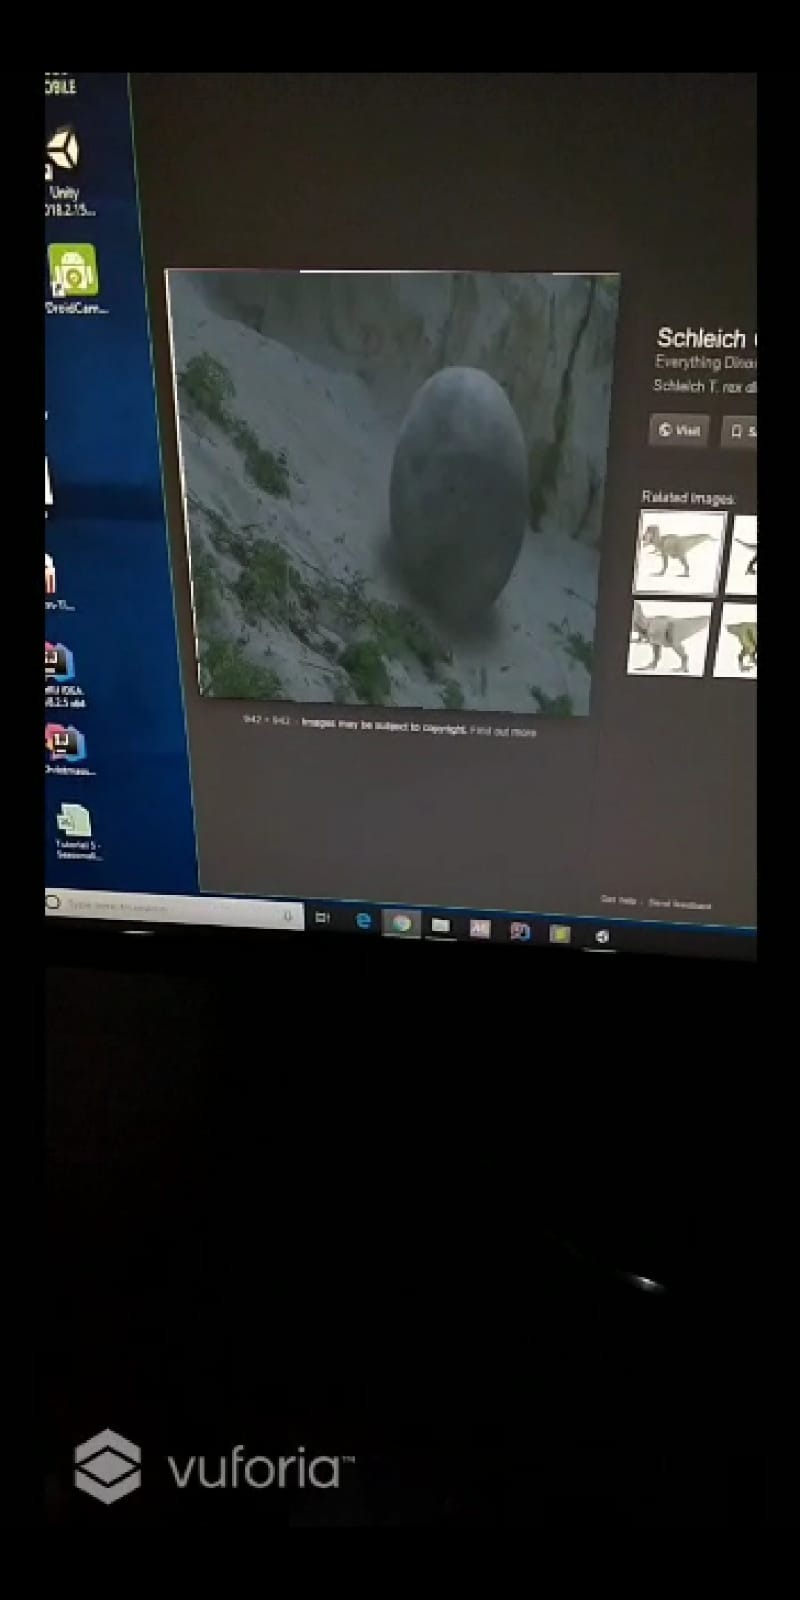
\includegraphics[width=60mm, height=100mm]{prototypes/ar/vulforia/2.jpeg} \\
(a) first & (b) second \\[6pt]
\end{tabular}
\caption{caption}
\end{figure}

\newpage
\subsubsection{ARKit}
\begin{figure}[H]
\centering  
\begin{tabular}{cc}
  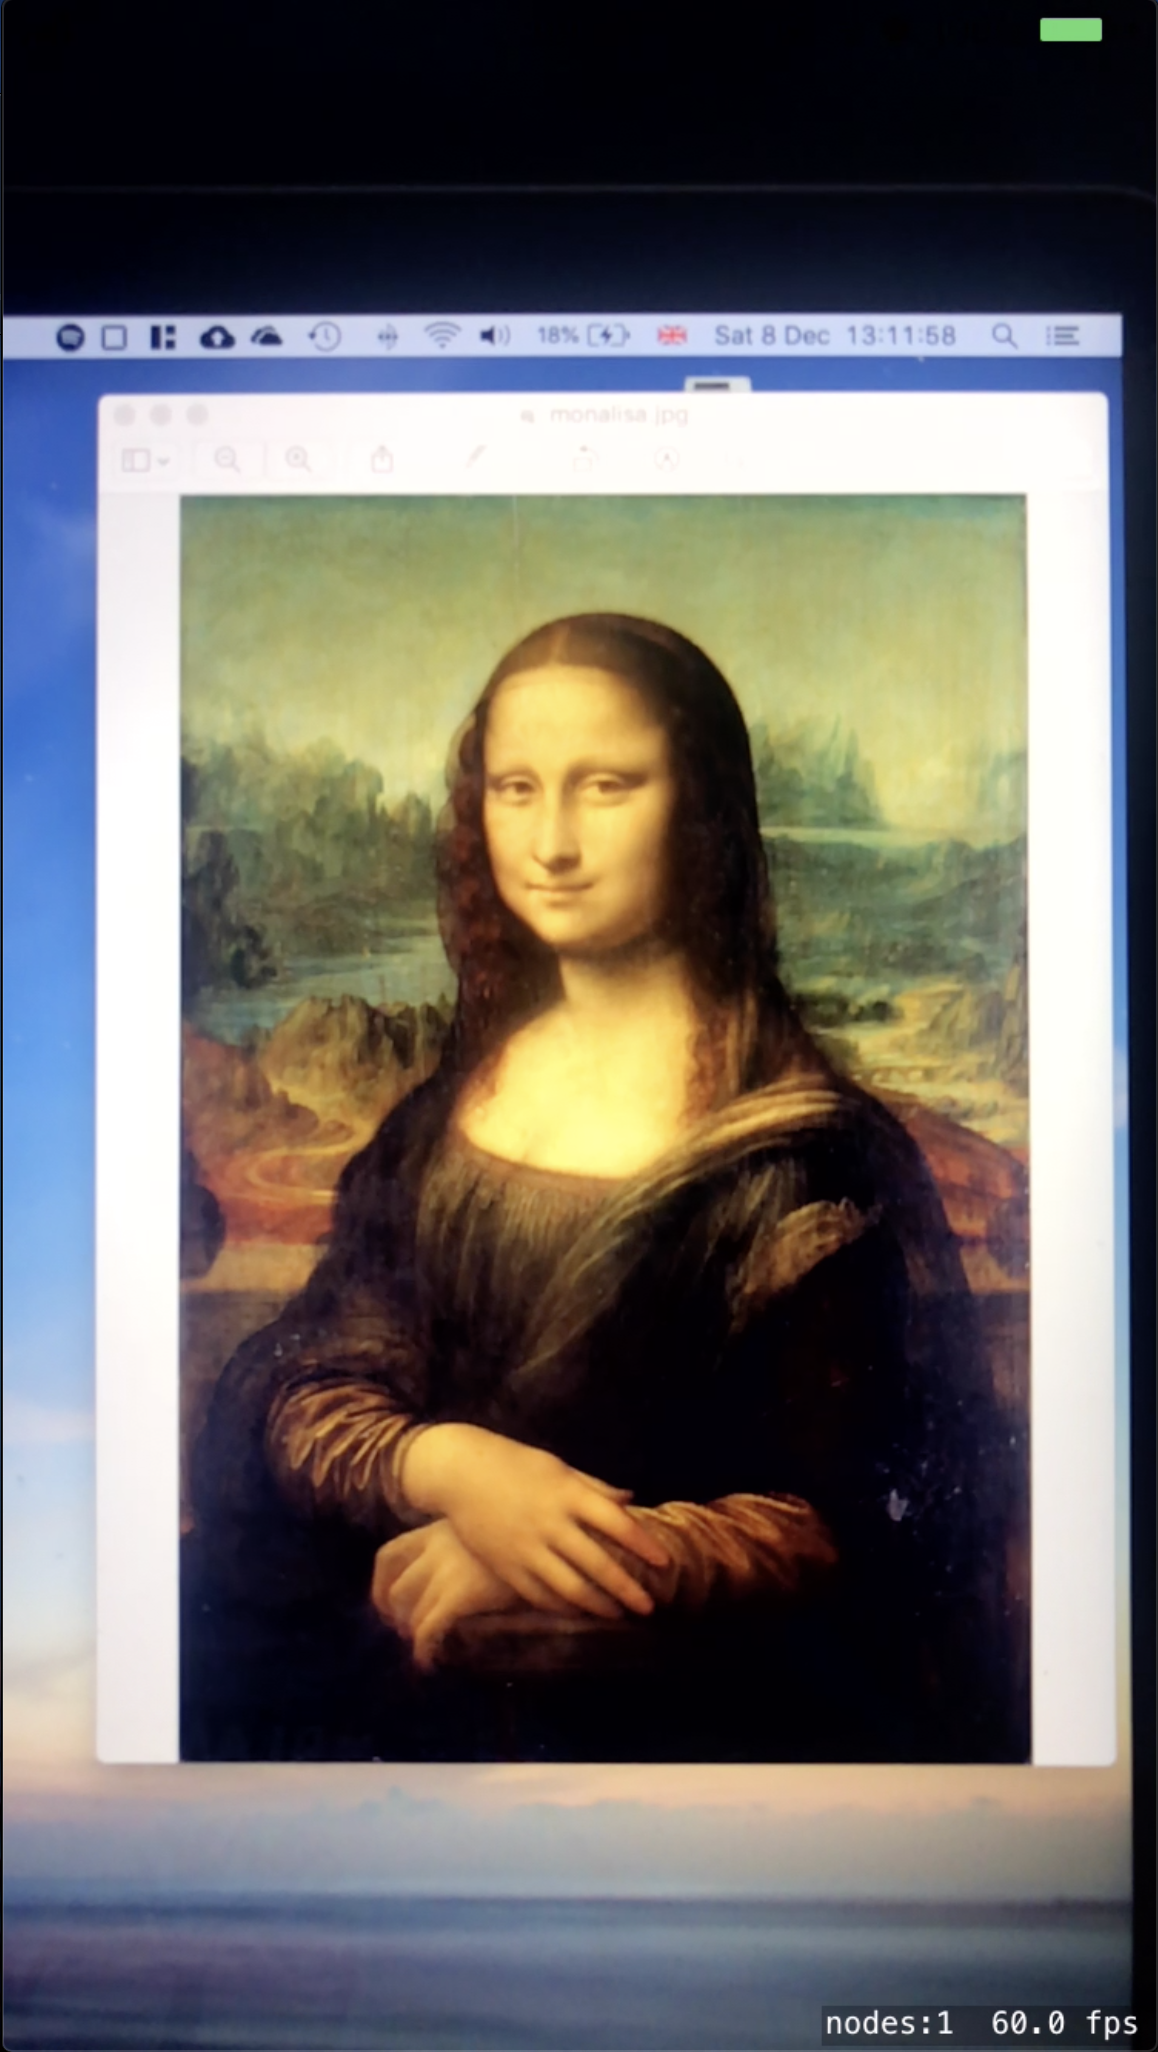
\includegraphics[width=60mm, height=100mm]{prototypes/ar/ios/1.png} &   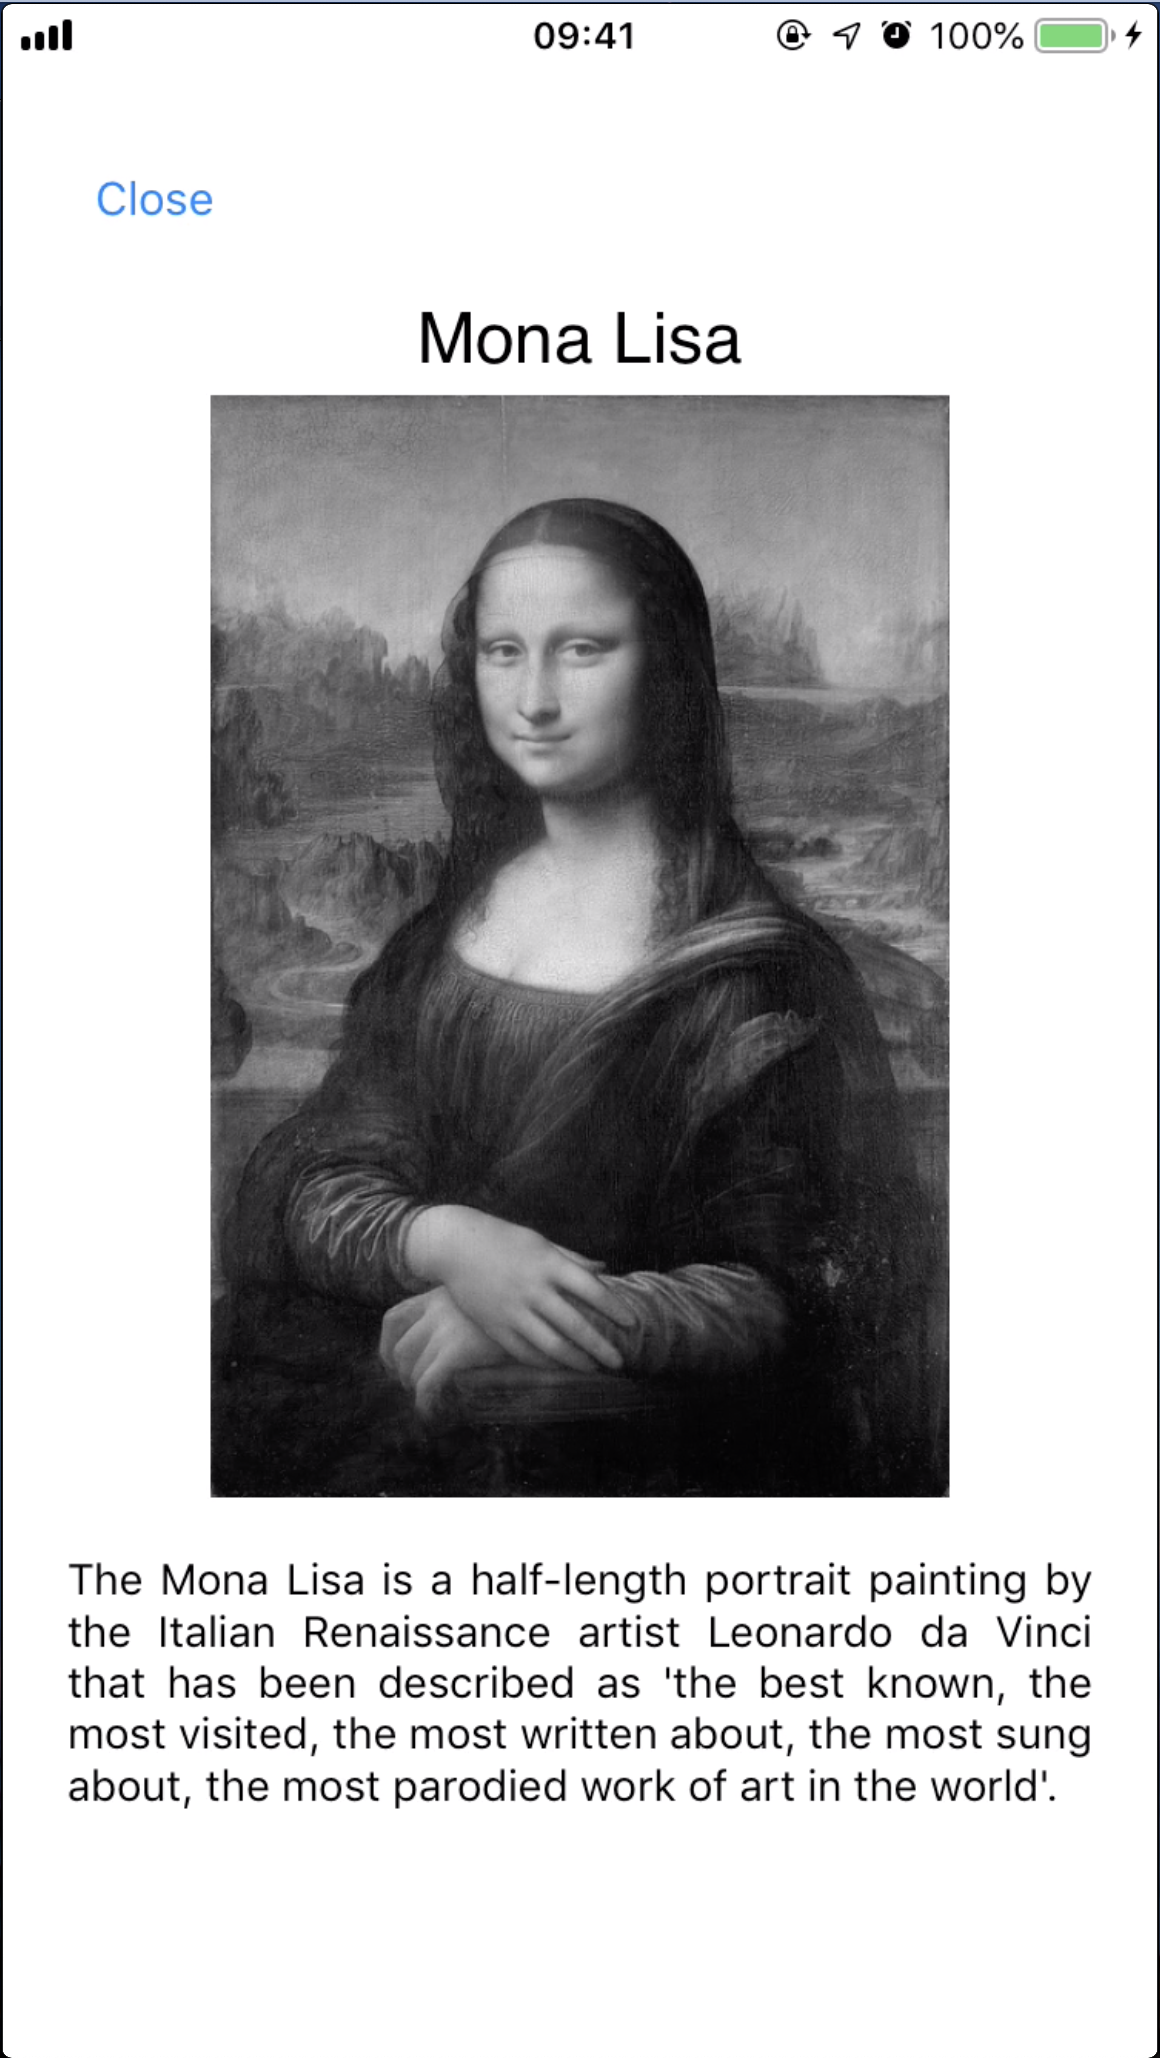
\includegraphics[width=60mm, height=100mm]{prototypes/ar/ios/2.png} \\
(a) first & (b) second \\[6pt]
\multicolumn{2}{c}{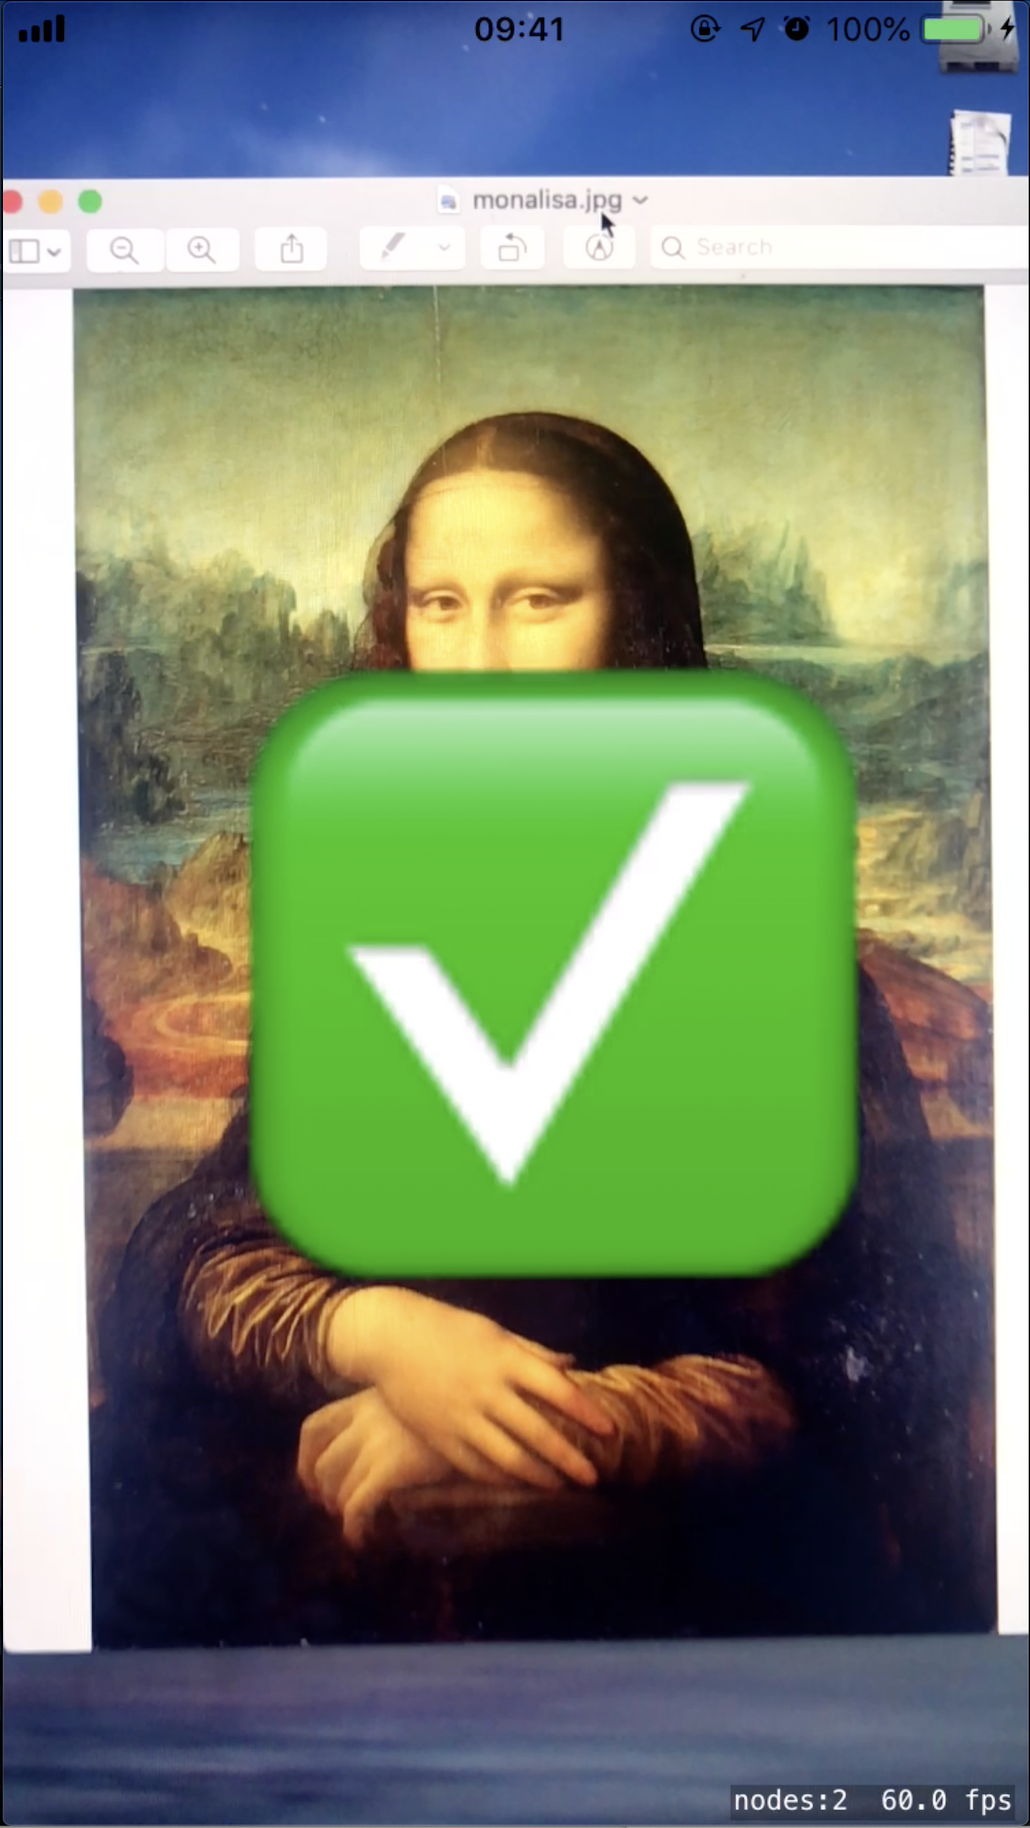
\includegraphics[width=60mm, height=100mm]{prototypes/ar/ios/3.png} }\\
\multicolumn{2}{c}{(e) fifth}
\end{tabular}
\caption{caption}
\end{figure}

\newpage
\subsubsection{ARCore}
\begin{figure}[H]
\centering  
\begin{tabular}{cc}
  
\includegraphics[width=60mm, height=100mm]{prototypes/ar/android/1.jpg} &   
\includegraphics[width=60mm, height=100mm]{prototypes/ar/android/2.jpg} \\
(a) first & (b) second \\[6pt]
\multicolumn{2}{c}{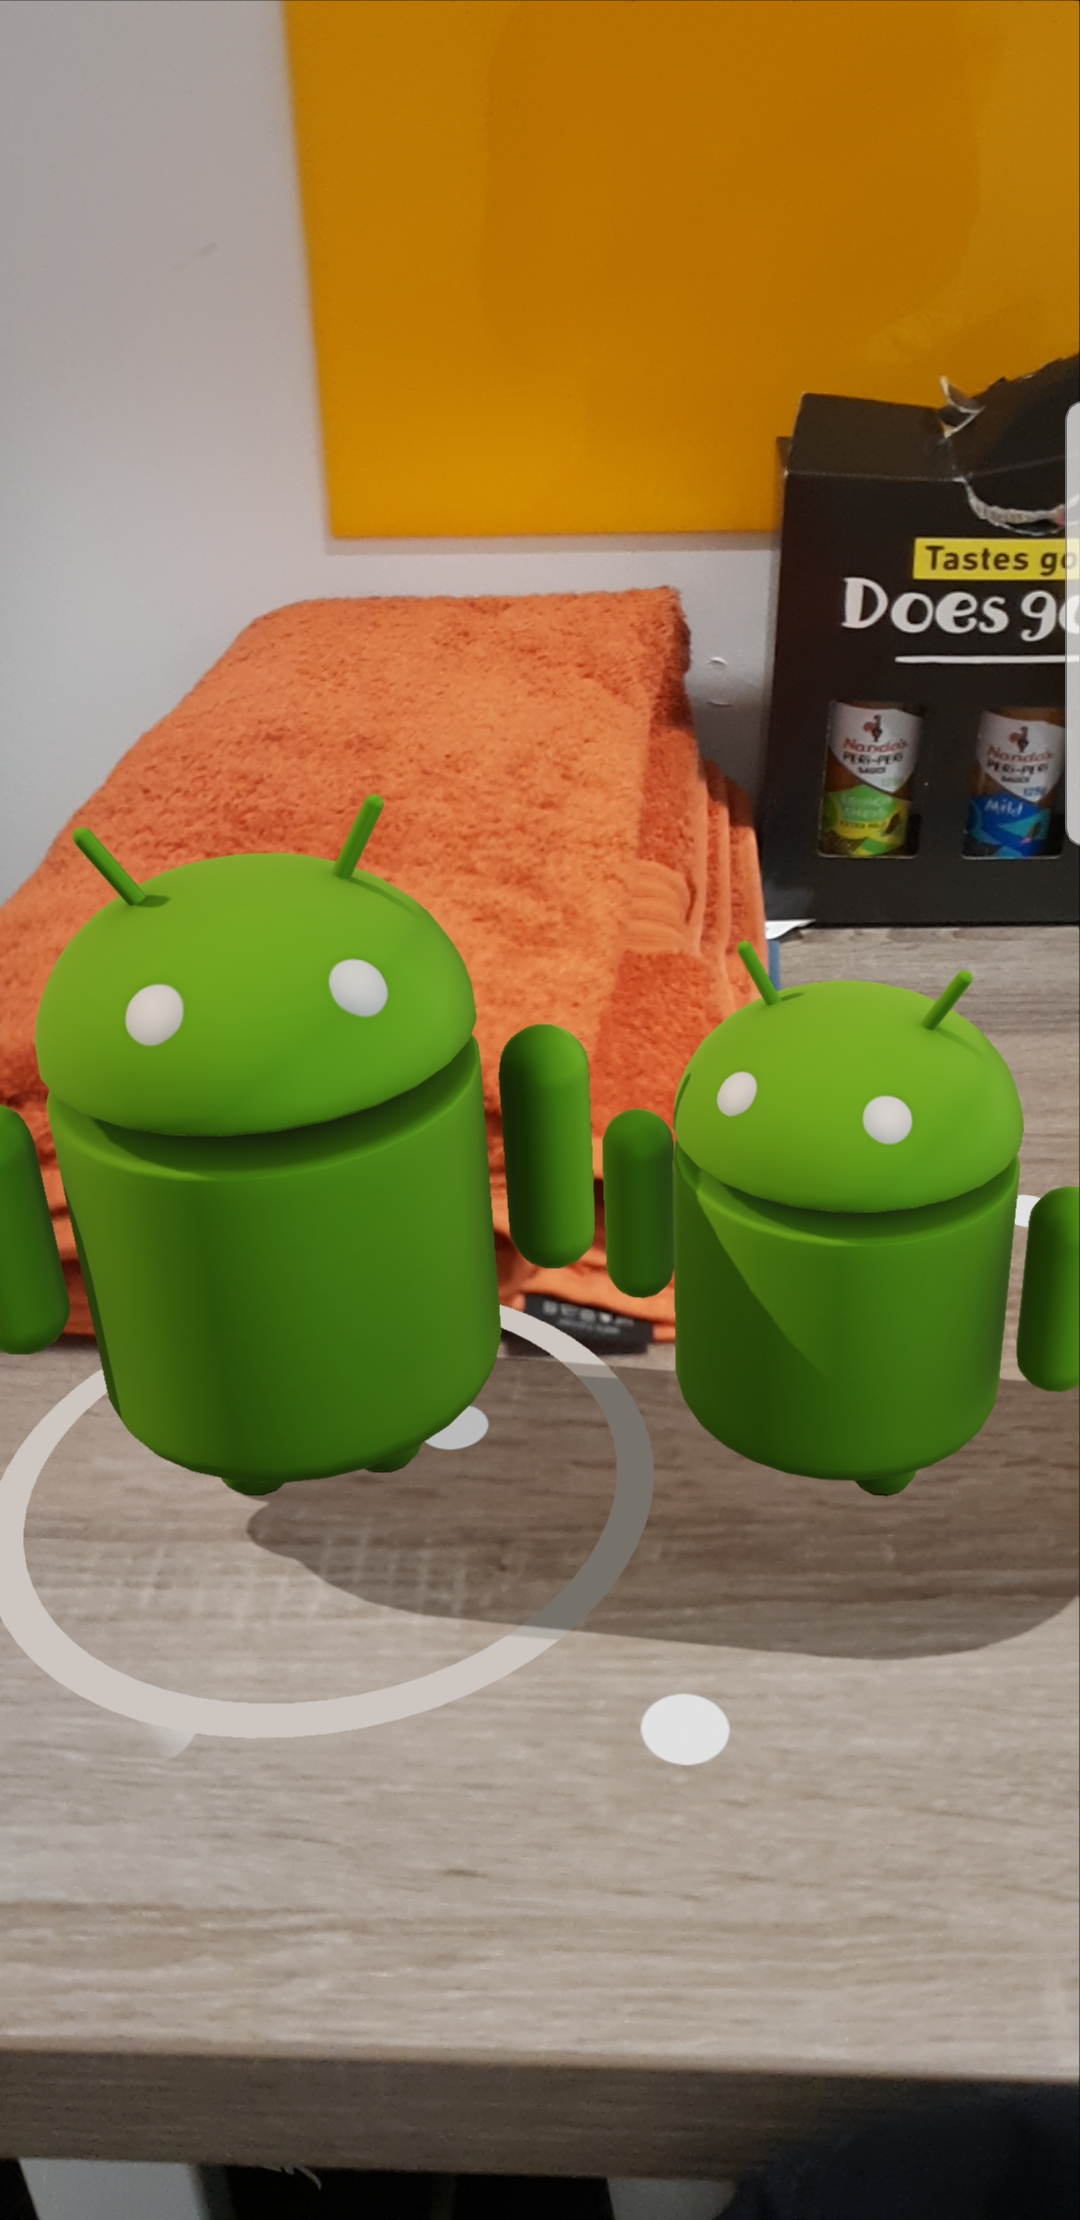
\includegraphics[width=60mm, height=100mm]{prototypes/ar/android/3.jpg} }\\
\multicolumn{2}{c}{(e) fifth}
\end{tabular}
\caption{caption}
\end{figure}

\newpage
\subsubsection{Android Sensors Logging}
\begin{figure}[H]
    \centering
    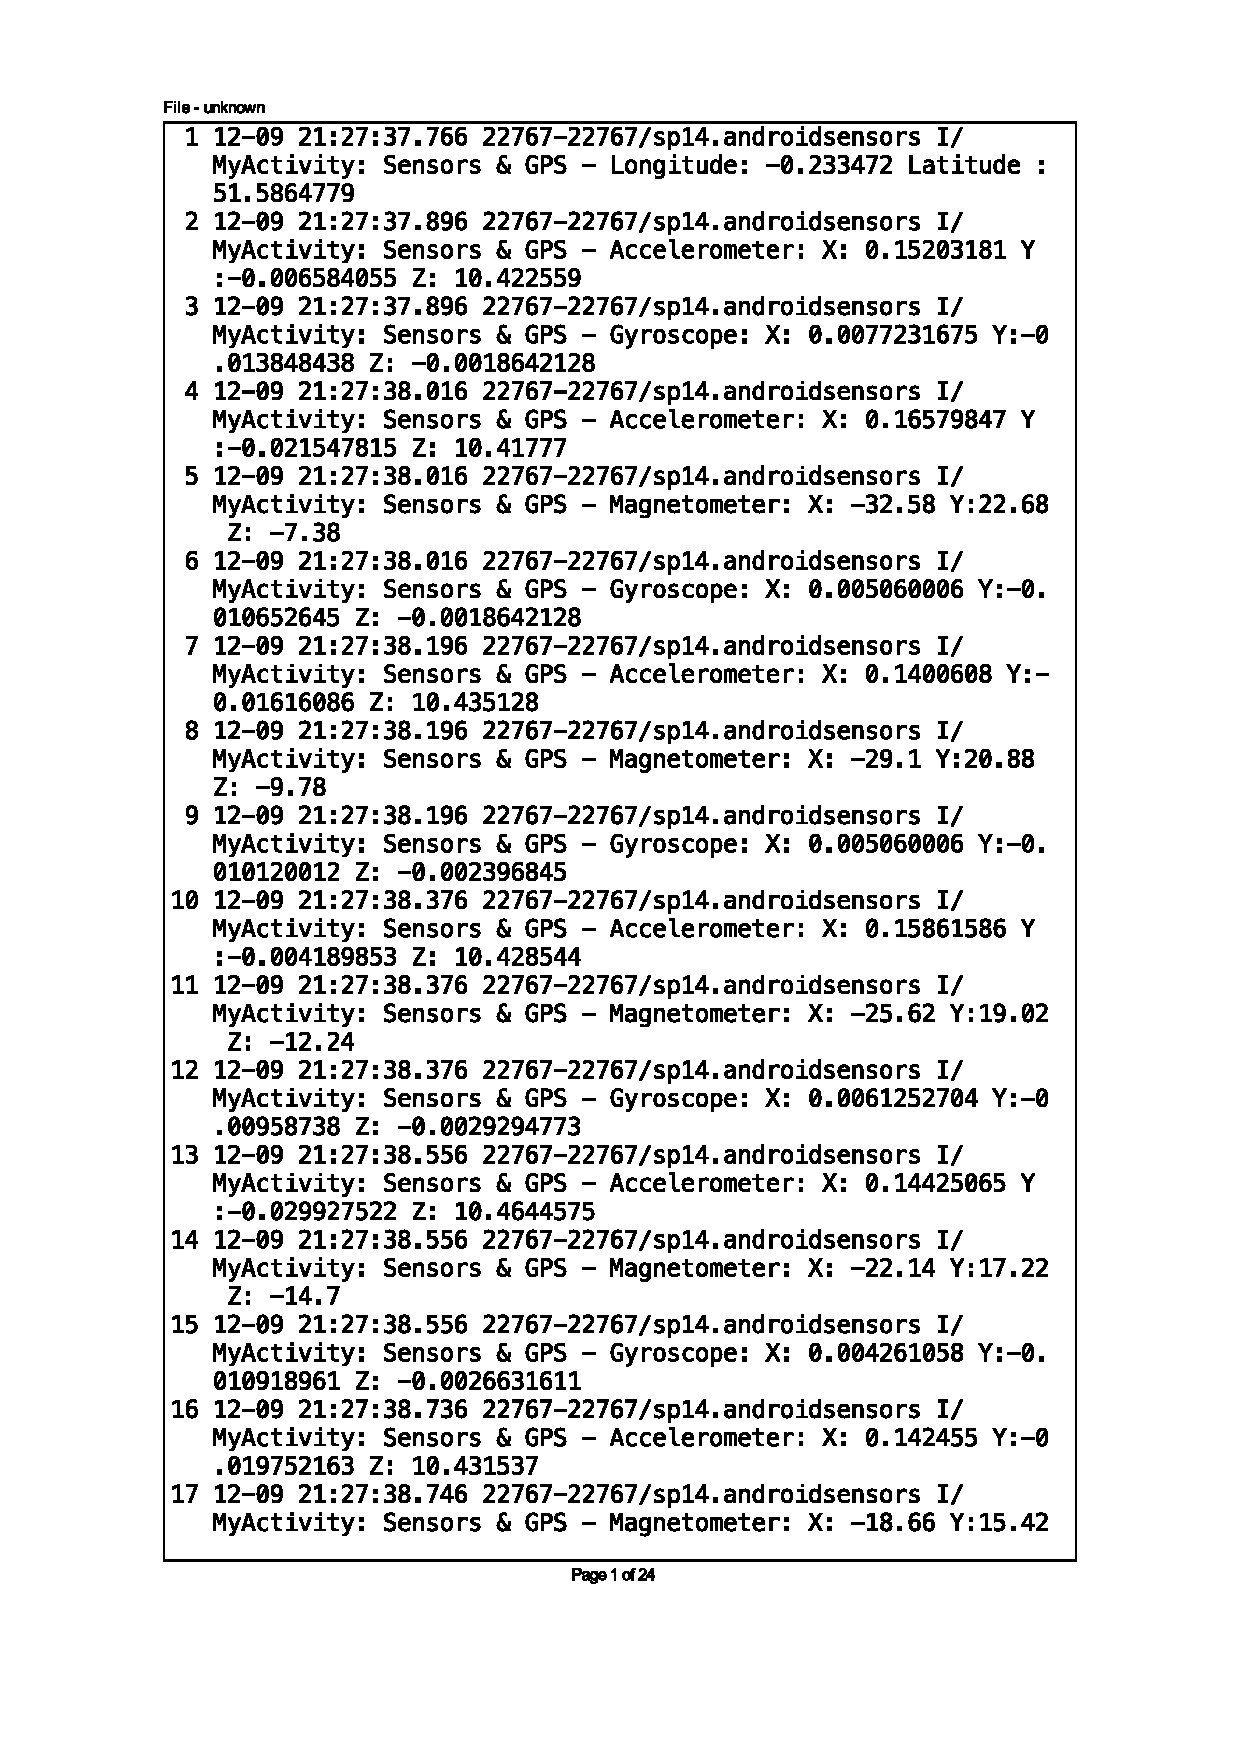
\includegraphics[width=\textwidth]
    {prototypes/ar/android/logs.pdf}
    \caption{Activity Model Diagram}
    \label{fig:Activity Model Diagram}
\end{figure}

\subsection{UI/UX Prototypes}
\subsubsection{Storyboard}
\begin{figure}[H]
    \centering
    \includegraphics[width=\textwidth]
    {prototypes/ui/storyboard.pdf}
    \caption{Storyboard}
    \label{fig:AtoB}
\end{figure}

\subsubsection{Prototype 1}
\begin{figure}[H]
    \centering
    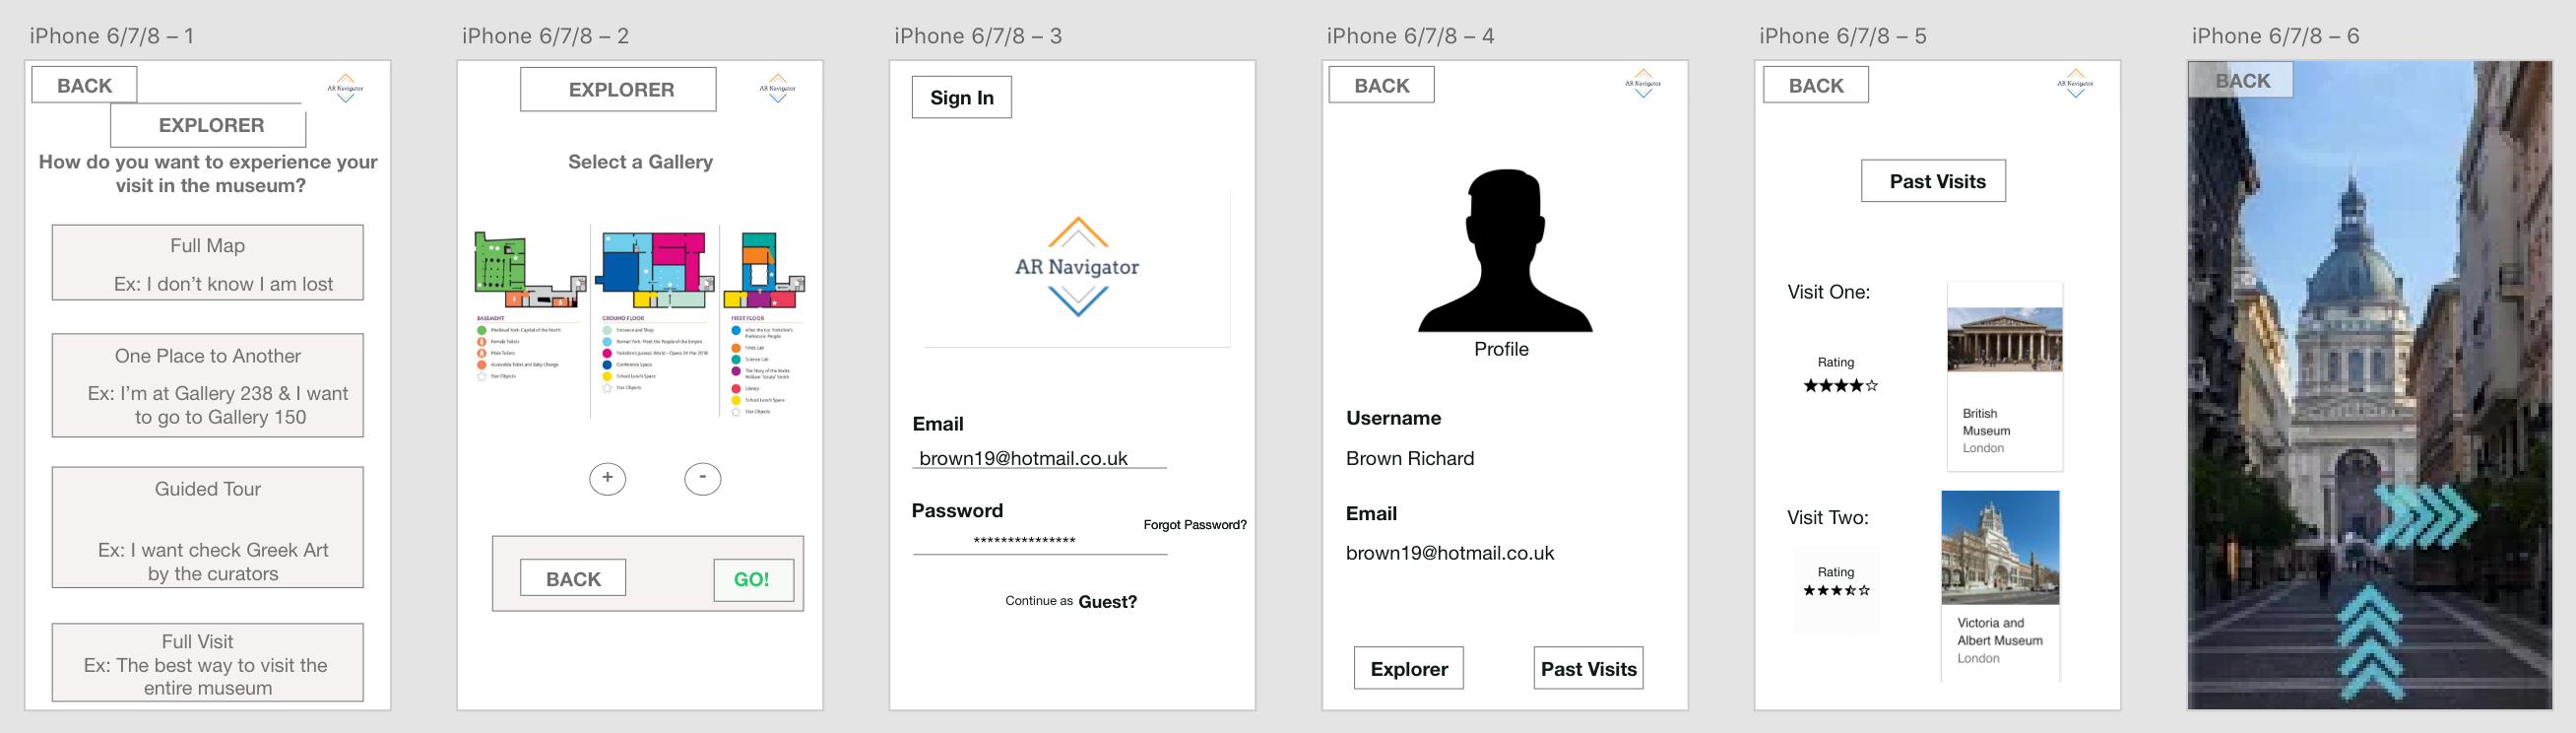
\includegraphics[width=\textwidth]
    {prototypes/ui/1.png}
    \caption{Overview of Prototype 1}
    \label{fig:prototype1}
\end{figure}

\subsubsection{Prototype 2}
\begin{figure}[H]
    \centering
    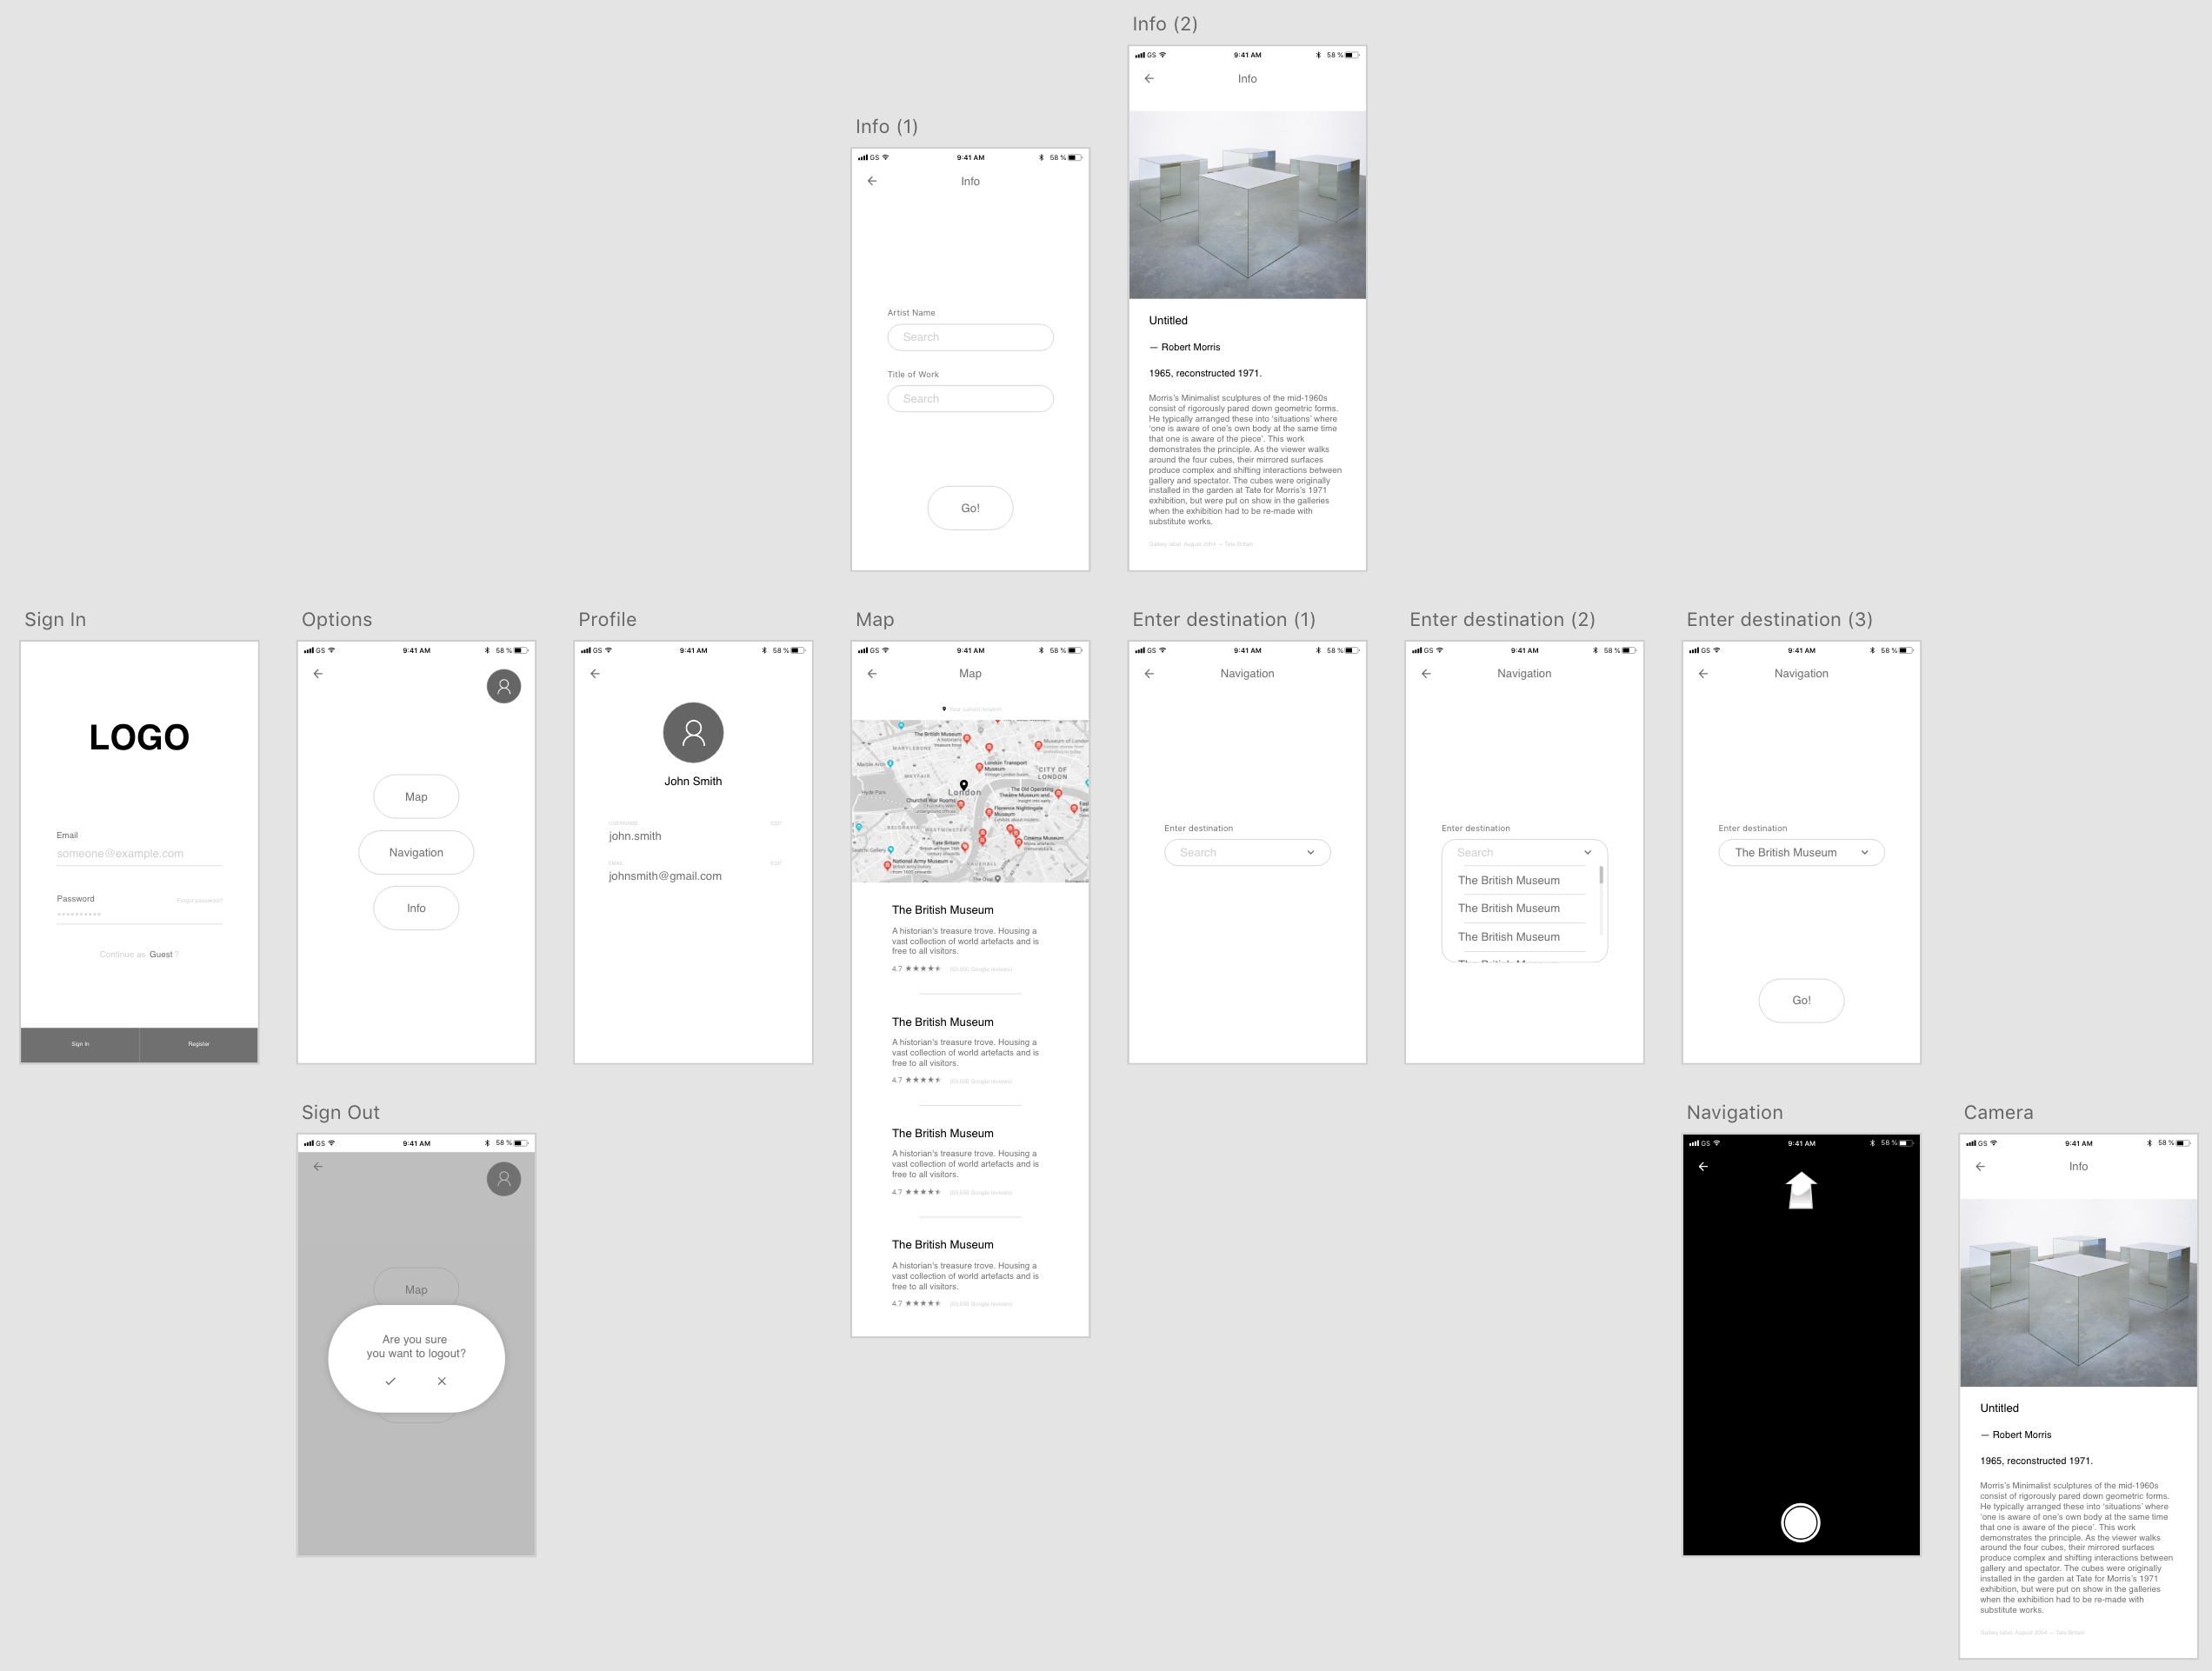
\includegraphics[width=\textwidth]
    {prototypes/ui/2.png}
    \caption{Overview of Prototype 2}
    \label{fig:prototype2}
\end{figure}

\subsubsection{Prototype 3}
\begin{figure}[H]
    \centering
    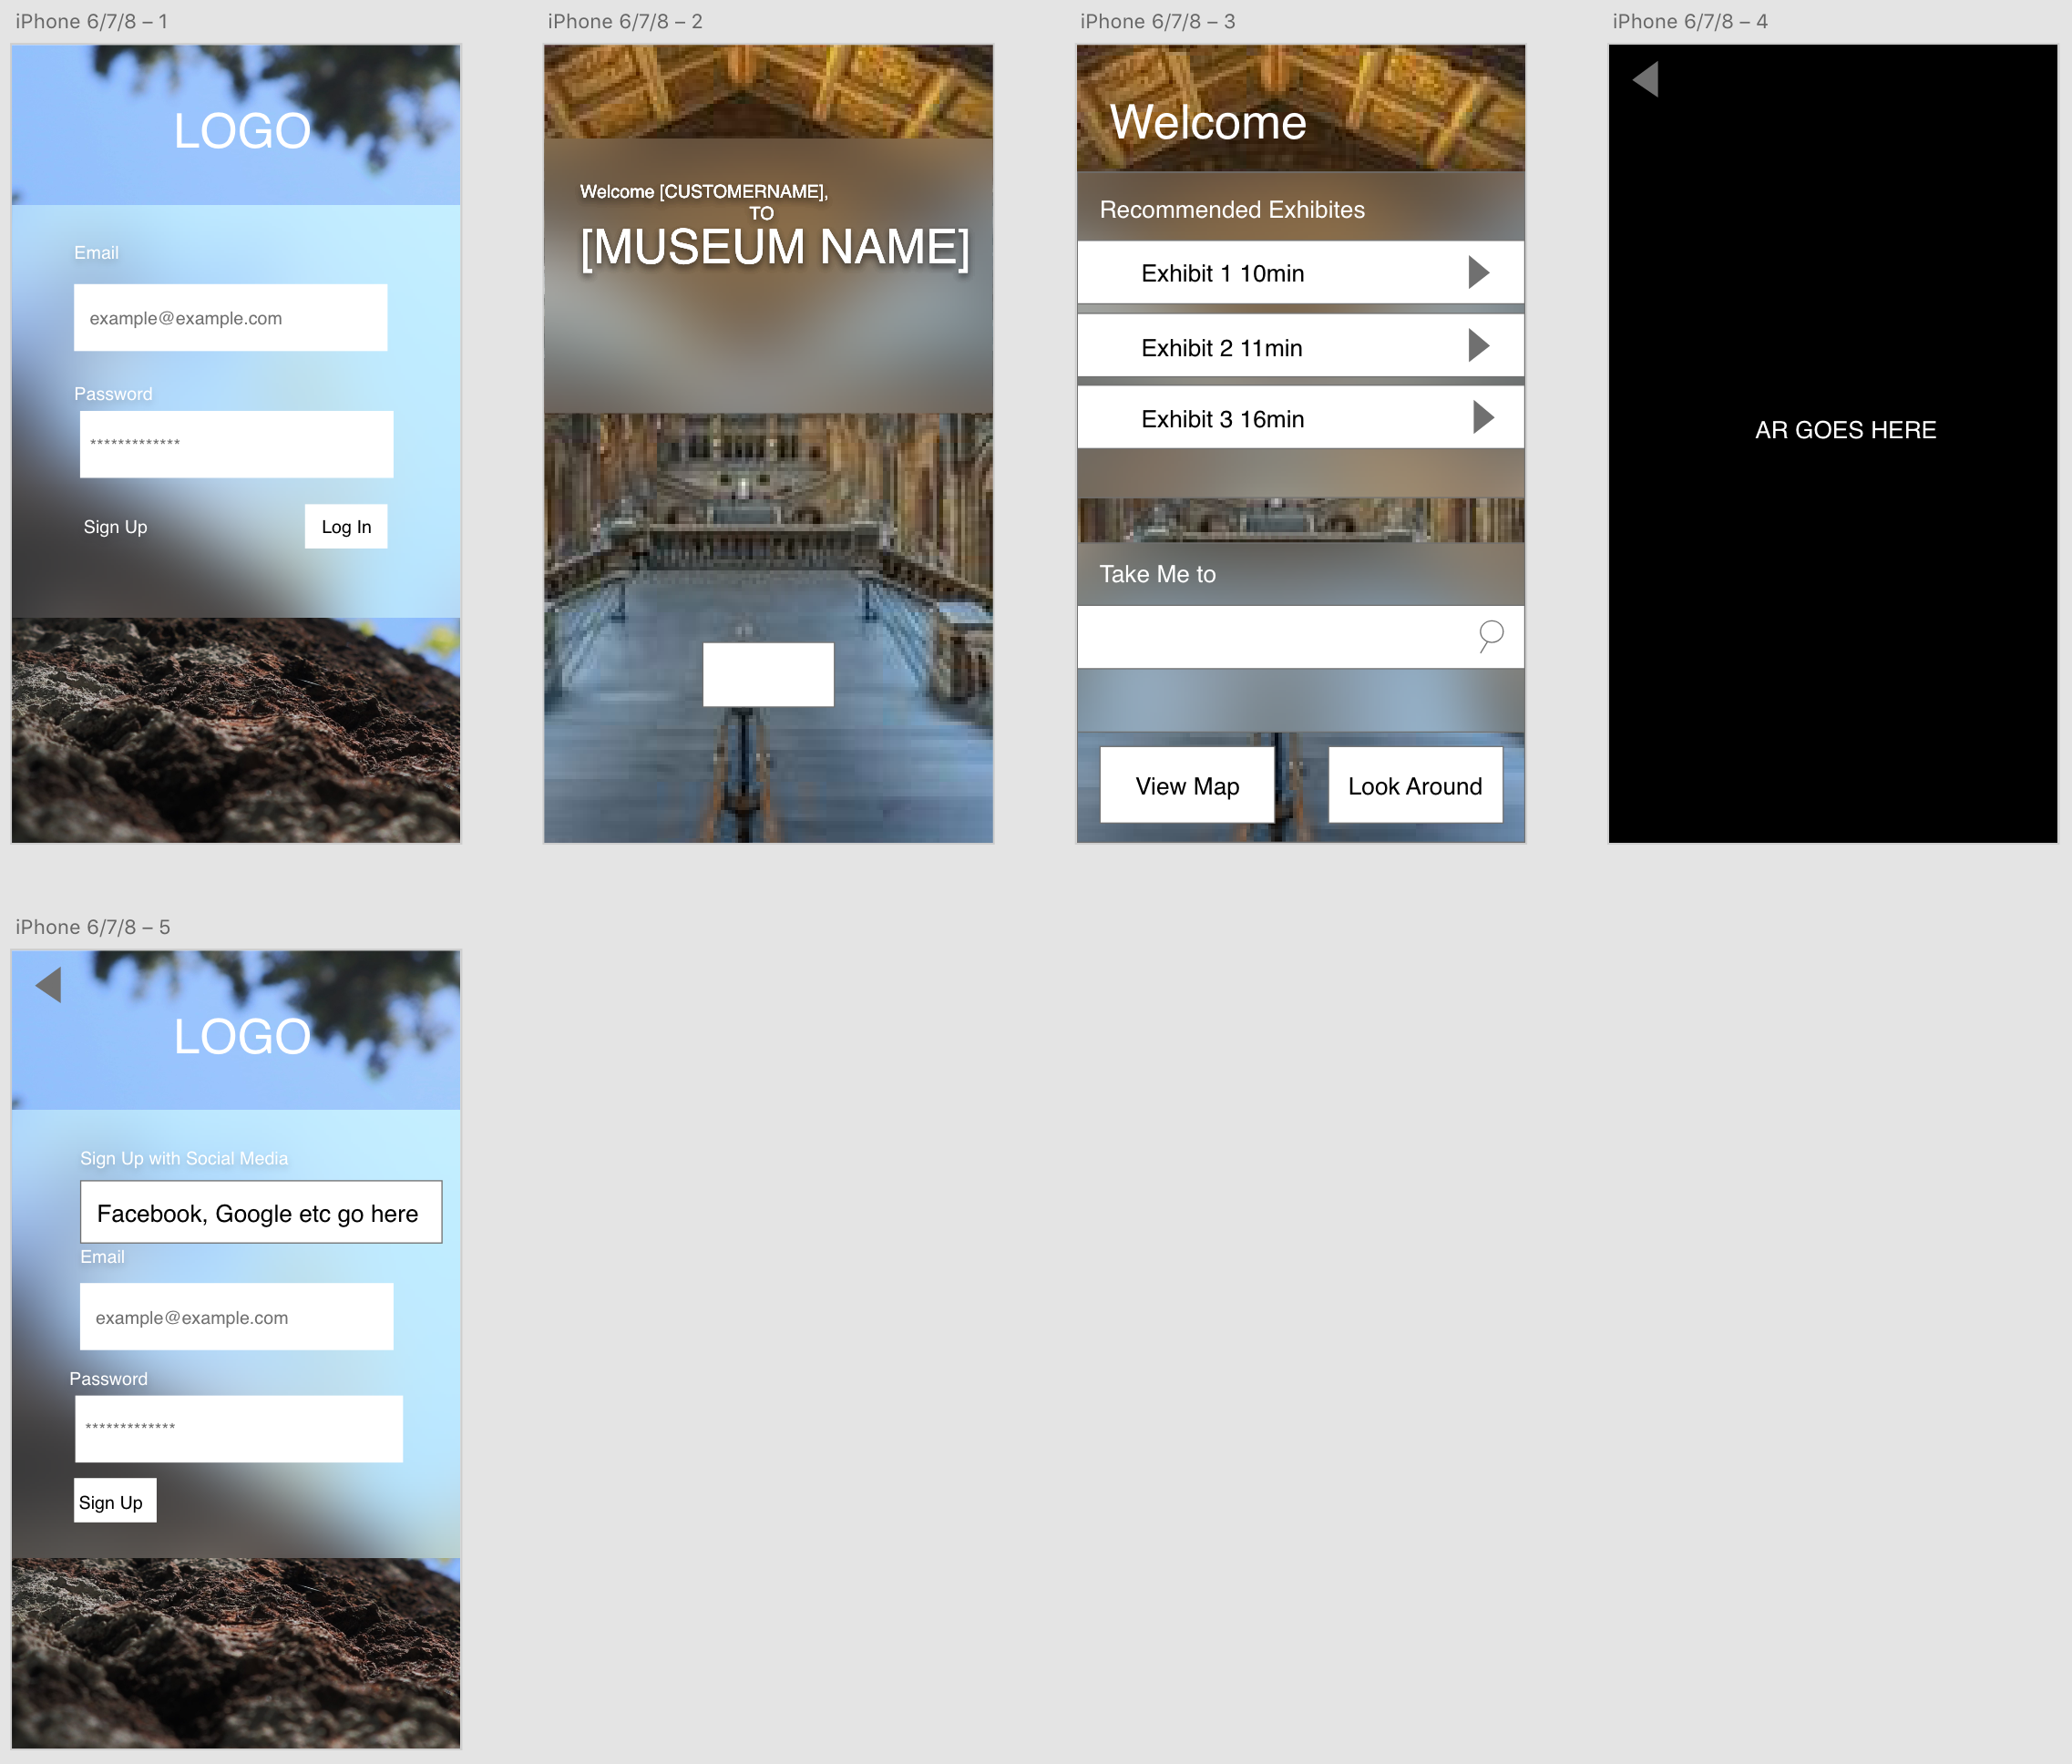
\includegraphics[width=\textwidth]
    {prototypes/ui/3.png}
    \caption{Overview of Prototype 3}
    \label{fig:prototype3}
\end{figure}

\newpage
\subsubsection{Prototype Reviews}
\textbf{Prototype 1}\\
This prototype again is very plain but this is made to look it was done so on purpose as it looks more professional and although the prototype has a lot of buttons, greatly considers the end user and what things we would want to do on the application making the potential of it greater. The search function and the map feature makes it a lot more personal to the user with potential options that they may select. Overall, because it considers the user more, this type of format at least should be used in the final version. One suggestion would be to maybe include colour as well as improve the logo because it is not very clear what the application is from looking at this, so have a logo to reflect this. The separate page for the use of AR is very good but one concern is how the the app will detect will where the user is or whether they can use the AR feature anywhere even without visiting the museum.\\

\textbf{Prototype 2}\\
The prototype at first glance looks very plain and with not much information or scope for the user to explore the app and seems very limited. One of the key things which could improve the app is simply to add colour to make it more appealing and engaging to users. Also, it is not very clear what the application is used for and how it can improve the existing method of visiting a museum - which I now know what the app’s purpose is - where a visitor can just have a guided tour from an expert or even an auditory tour. Certain features of the prototype were good such as the search feature and the clarity making the app user-friendly. As well as this, the fact that the app shows the closest museum to the input given is very helpful, showing the rating given by visitors making easier to choose which museum to visit. The fact that it also has logout confirmation page and a page showing the users account where they can add favourite museums and add ratings and reviews gives other users better choice where they can make a more informed decision.\\

\textbf{Prototype 3}\\
The prototype is quite plain at first glance although the use of colour through use of the background is good. It is more appealing and engaging. However, use of the application seems very basic and limited with little function. The prototype consists mainly of buttons and doesn’t allow much user input, that being said, the search function is a good addition. Overall, this prototype is very limited and use of the prototype 2 should be used over this one.

\newpage
\subsubsection{Final Prototype}
\begin{figure}
\begin{tabular}{cc}
  \includegraphics[width=65mm]{it} &   \includegraphics[width=65mm]{it} \\
(a) first & (b) second \\[6pt]
 \includegraphics[width=65mm]{it} &   \includegraphics[width=65mm]{it} \\
(c) third & (d) fourth \\[6pt]
\end{tabular}
\caption{caption}
\end{figure}

\newpage
\section{Technical Architecture}
% \subsection{Backlog}
\begin{figure}[H]
    \centering
    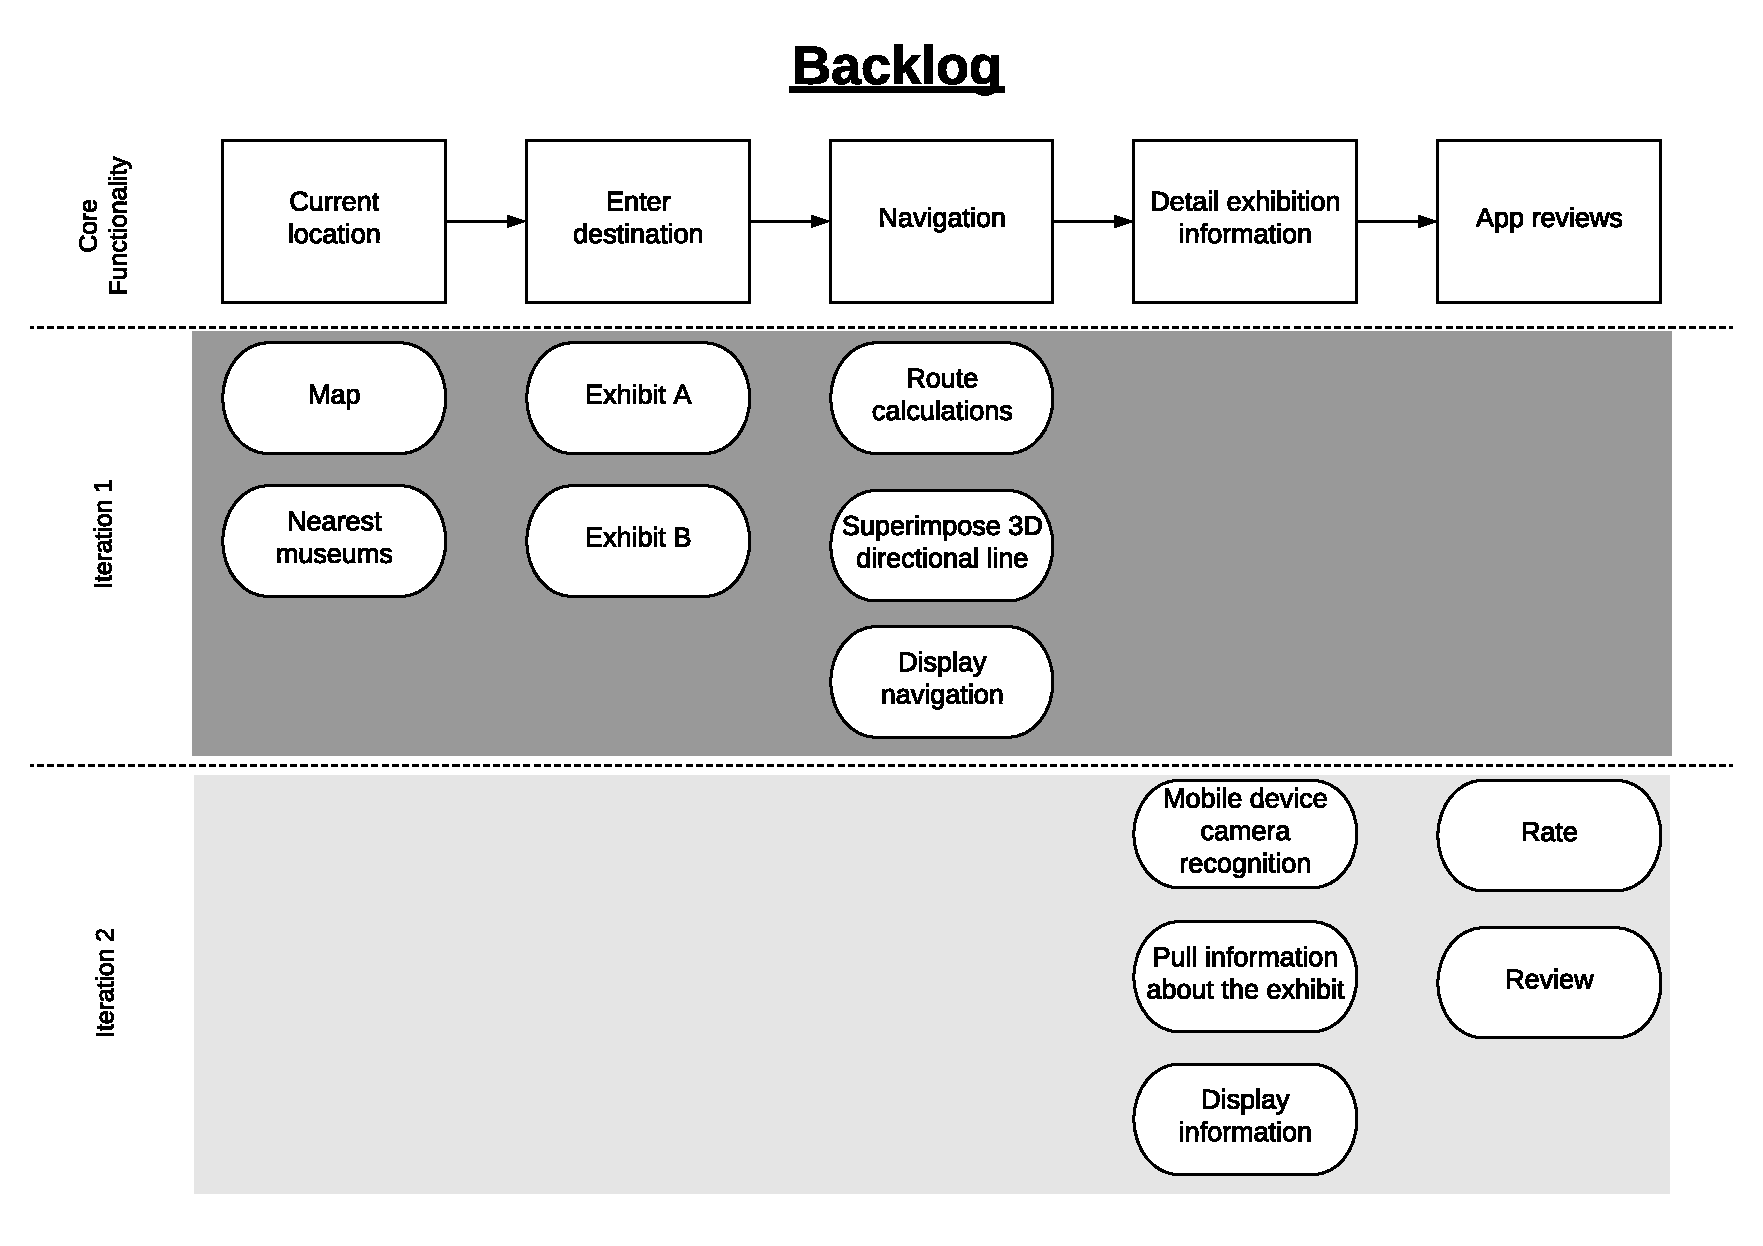
\includegraphics[width=\textwidth]
    {technicalarchitecture/backlog.pdf}
    \caption{Activity Model Diagram}
    \label{fig:Activity Model Diagram}
\end{figure}

% \subsection{MVC}
\begin{figure}[H]
    \centering
    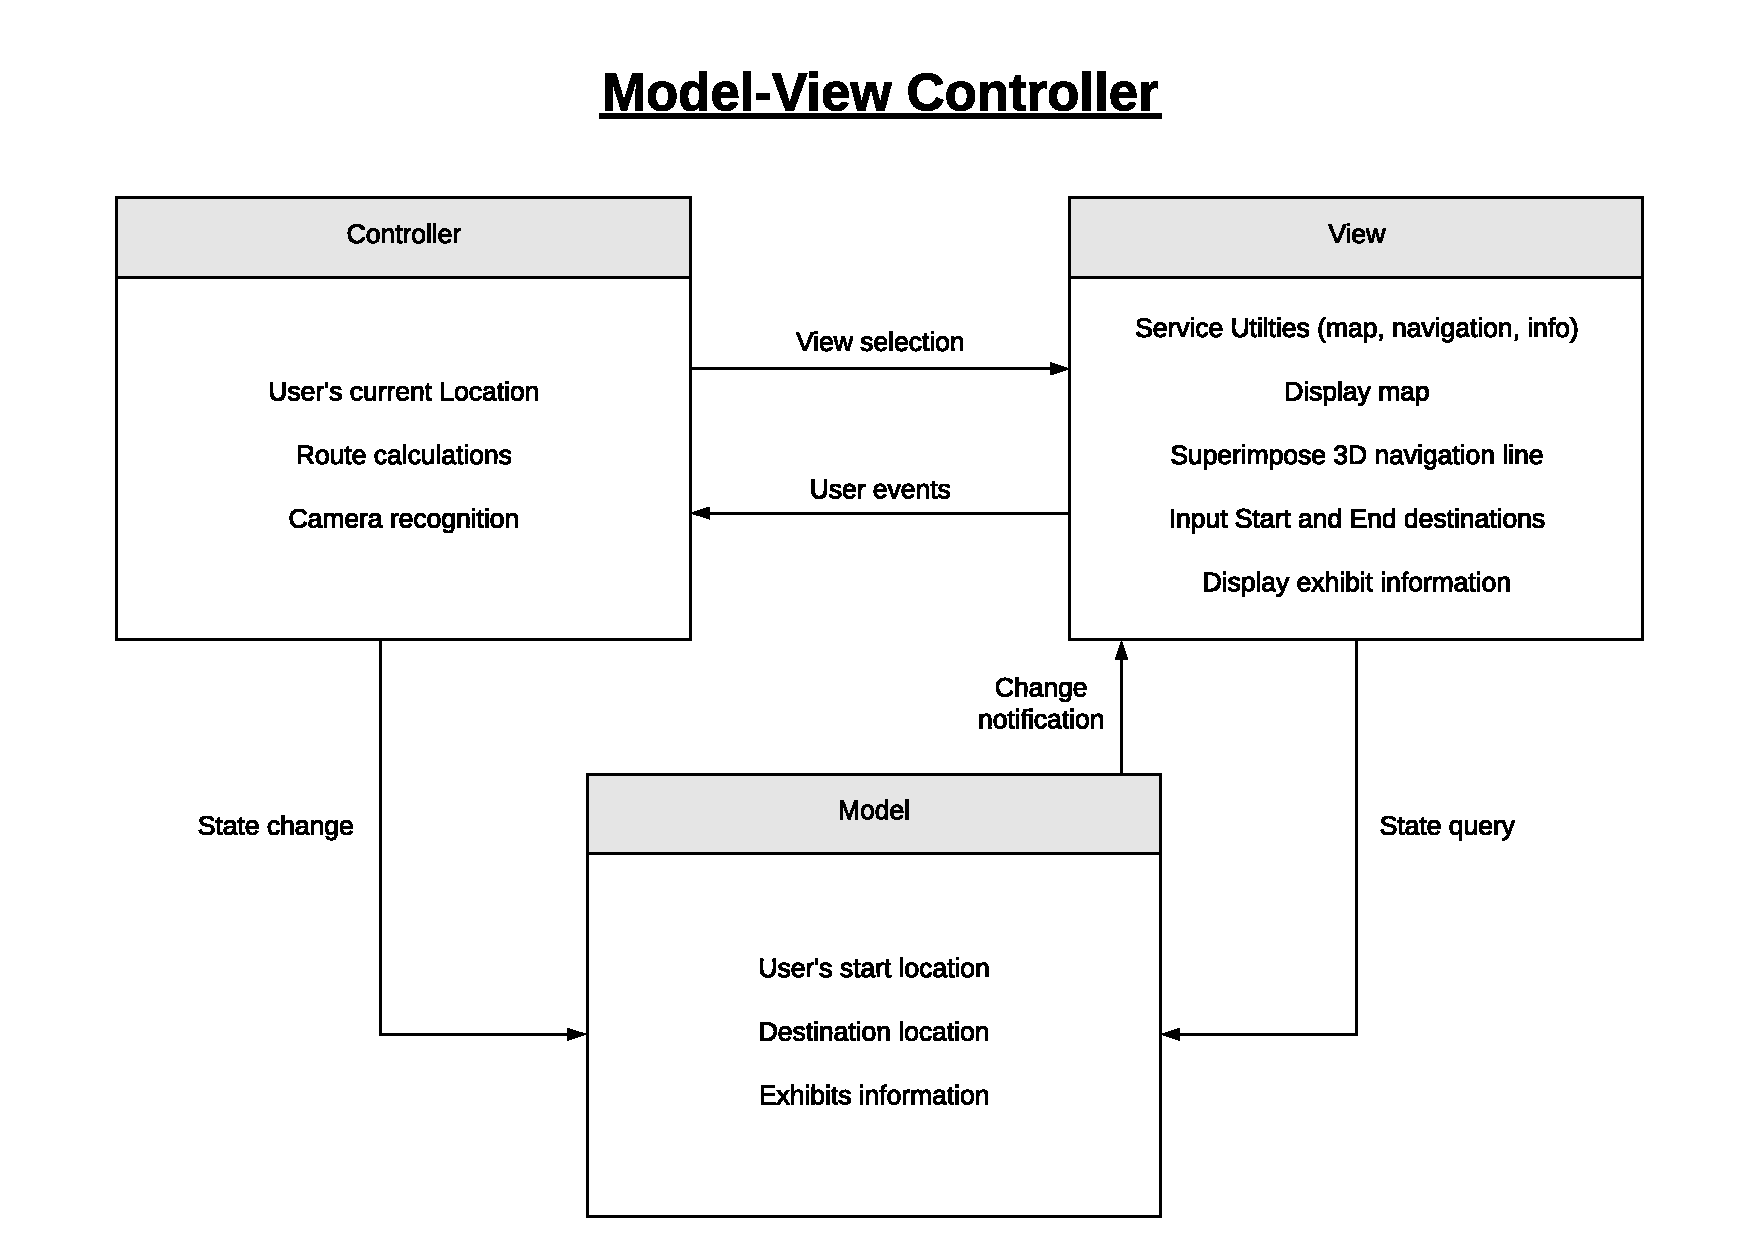
\includegraphics[width=\textwidth]
    {technicalarchitecture/mvc.pdf}
    \caption{Activity Model Diagram}
    \label{fig:Activity Model Diagram}
\end{figure}


\chapter{Prototype Reviews} \label{Prototype Reviews}
\section*{Prototype 1}
This prototype again is very plain but this is made to look it as it looks more professional and although the prototype has a lot of buttons, this greatly considers the end user and what things we would want to do on the application making the potential of it greater. The search function and the map feature makes it a lot more personal to the user with potential options that they may select. Overall, because it considers the user more, this type of format at least should be used in the final version. One suggestion would be to maybe include colour as well as improve the logo because it is not very clear what the application is from looking at this, so have a logo to reflect this. The separate page for the use of AR is very good but one concern is how the the app will detect will where the user is or whether they can use the AR feature anywhere even without visiting the museum.\\

\section*{Prototype 2}
The prototype at first glance looks very plain and with not much information or scope for the user to explore the app and seems very limited. One of the key things which could improve the app is simply to add colour to make it more appealing and engaging to users. Also, it is not very clear what the application is used for and how it can improve the existing method of visiting a museum - which I now know what the app’s purpose is - where a visitor can just have a guided tour from an expert or even an auditory tour. Certain features of the prototype were good such as the search feature and the clarity making the app user-friendly. As well as this, the fact that the app shows the closest museum to the input given is very helpful, showing the rating given by visitors making easier to choose which museum to visit. The fact that it also has logout confirmation page and a page showing the users account where they can add favourite museums and add ratings and reviews gives other users better choice where they can make a more informed decision.\\

\section*{Prototype 3}
The prototype is quite plain at first glance although the use of colour through the background is good. It is more appealing and engaging. However, use of the application seems very basic and limited with little function. The prototype consists mainly of buttons and doesn’t allow much user input, that being said, the search function is a good addition. Overall, this prototype is very limited and use of the prototype 2 should be used over this one.


\afterpage{\blankpage}
\chapter{Meeting Minutes}
\section*{Structure}
Academic weeks are indicated in brackets.\\

All weekly meetings are structured as:
\begin{itemize}
	\item Monday (in person) - Lab sprint planning
	\item Thursday (virtual) - Team sprint review
	\item Friday (in person) - Project supervisor meeting
\end{itemize}

\section*{Week 1 (1)}
\subsection*{Thursday 4 October 2018}
\begin{itemize}
	\item Meeting all team members
	\item Discussing potential concepts
\end{itemize}

\section*{Week 2 (2)}
\subsection*{Monday 8 October 2018}
\begin{itemize}
	\item Reviewing potential concepts discussed
    \item Considering stakeholders
\end{itemize}

\subsection*{Thursday 11 October 2018}
\begin{itemize}
	\item Reviewing project concept
\end{itemize}

\subsection*{Friday 12 October 2018}
\begin{itemize}
    \item Submission of project tracking form
	\item Meeting project supervisor
	\item Submission of project concept
\end{itemize}

\section*{Week 3 (3)}
\subsection*{Monday 15 October 2018}
\begin{itemize}
    \item Updating project tracking form
	\item Tweaking project concept to be museum focused 
	\item Creating scrum board to track tasks
	\item Allocating market research
    \item Creating stakeholder requirements activities
	\item Allocating questionnaire
\end{itemize}

\subsection*{Thursday 18 October 2018}
\begin{itemize}
	\item Updating project tracking form
	\item Reviewing market research
	\item Reviewing questionnaire
\end{itemize}

\subsection*{Friday 19 October 2018}
\begin{itemize}
    \item Submission of project tracking form
	\item Submission of market research
	\item Submission of questionnaire
	\item Further research on different stakeholders of different demographics suggested by project supervisor
\end{itemize}

\section*{Week 4 (4)}
\subsection*{Monday 22 October 2018}
\begin{itemize}
    \item Building use sequence model
	\item Allocating activity model
	\item Allocating service model
\end{itemize}

\subsection*{Thursday 25 October 2018}
\begin{itemize}
	\item Updating project tracking form
	\item Reviewing use sequence model
	\item Reviewing activity model
	\item Reviewing service model 
\end{itemize}

\subsection*{Friday 26 October 2018}
\begin{itemize}
    \item Submission of project tracking form
	\item Submission of all models
	\item Updating supervisor on team collaboration
\end{itemize}

\section*{Week 5 (5)}
\subsection*{Monday 29 October 2018}
\begin{itemize}
    \item Creating open questions
	\item Allocating storyboard
	\item Creating outline for proposal
	\item Creating Gantt chart
	\item Allocating UI/UX prototyping
	\item Allocating AR libraries investigation
\end{itemize}

\subsection*{Thursday 1 November 2018}
\begin{itemize}
	\item Reviewing storyboard
	\item Reviewing project tracking form
\end{itemize}

\subsection*{Friday 2 November 2018}
\begin{itemize}
    \item Showed our storyboard
    \item Submission of project tracking form
	\item Updating supervisor on storyboards and current prototyping
	\item Collate all half term work in one document and send to supervisor
\end{itemize}

\section*{Week 7 (Reading week)}
\subsection*{Thursday 8 November 2018}
\begin{itemize}
	\item Gathering raw stakeholder research information
	\item Analysis and review on raw stakeholder research
	\item Updating project tracking form
\end{itemize}

\section*{Week 7 (6)}
\subsection*{Monday 12 November 2018}
\begin{itemize}
	\item Reviewing Gantt chart
    \item Reviewing open questions
    \item Reviewing stakeholder research
    \item Creating plans for stakeholders using prototypes
    \item Peer-reviewing of UI/UX prototypes
\end{itemize}

\subsection*{Monday 13 November 2018}
\begin{itemize}
	\item Do research on Stakeholder
\end{itemize}

\subsection*{Thursday 15 November 2018}
\begin{itemize}
    \item Updating project tracking form
	\item Review of the peer-reviews
	\item Start with UI/UX prototypes
	\item Research on Android/iOS platforms
\end{itemize}

\subsection*{Friday 16 November 2018}
\begin{itemize}
    \item Submission of project tracking form
	\item Demonstrating individual UI/UX prototypes to supervisor
	\item Demonstrating each AR library research to supervisor
\end{itemize}

\section*{Week 8 (7)}
\subsection*{Monday 19 November 2018}
\begin{itemize}
	\item Reviewing Gantt chart
	\item Reviewing research on Android/iOS platform
	\item Building final UI/UX prototypes
\end{itemize}

\subsection*{Thursday 22 November 2018}
\begin{itemize}
    \item Updating project tracking form
	\item Review final android prototype
	\item Review final UX/UI prototype
\end{itemize}

\subsection*{Friday 23 November 2018}
\begin{itemize}
    \item Submission of project tracking form
	\item Presentation on everything completed so far to project supervisor
	\item Submission of all prototypes
\end{itemize}

\section*{Week 9 (8)}
\subsection*{Monday 26 November 2018}
\begin{itemize}
	\item Reviewing Gantt chart
	\item Allocating backlog
	\item Allocating open questions
	\item Allocating MVC
	\item Reviewing functional specification chapter
\end{itemize}

\subsection*{Thursday 29 November 2018}
\begin{itemize}
	\item Updating project tracking form
	\item Reviewing backlog
	\item Reviewing open questions so far
	\item Reviewing design chapter
\end{itemize}

\subsection*{Friday 30 November 2018}
\begin{itemize}
	\item Submission of project tracking form
	\item Presentation of open questions
	\item Presentation of backlog
	\item Spoken about fuse comapany
	\item Progress of framework of technical architecture
	\item Finish user stories by next week
	\item Finish off technical architecture (milestone) by next week
\end{itemize}

\section*{Week 10 (9)}
\subsection*{Monday 3 December 2018}
\begin{itemize}
	\item Reviewing Gantt chart
	\item Reviewing backlog, open questions, and MVC
	\item Reallocating chapters 5, 6, 7, 8 of proposal due to change in guidelines
	\item Reallocating user stories
	\item Preparation for concept presentation
\end{itemize}

\subsection*{Thursday 6 December 2018}
\begin{itemize}
	\item Updating project tracking form
\end{itemize}

\subsection*{Friday 7 December 2018}
\begin{itemize}
	\item Submission of project tracking form
	\item Submittted technical architecture work
	\item Decribed what we have include in technical architecture
	\item One to one discussion for how things are going within the group
	\item Explanation about open questions, backlog, MPV and user stories
	\item Discuss about 5 minutes presentation which going to take place on monday next week
\end{itemize}

\section*{Week 11 (10)}
\subsection*{Monday 10 December 2018}
\begin{itemize}
	\item Reviewing Gantt chart
\end{itemize}

\subsection*{Wednesday 12 December 2018}
\begin{itemize}
	\item Proof reading all chapters
	\item Writing abstract and conclusion of proposal
	\item Completion of meeting minutes
	\item Submission of proposal
\end{itemize}


\end{appendices}

%-----------------------
% BIBLIOGRAPHY
%-----------------------
% \bibliographystyle{unsrt}
% \bibliography{references}
\addcontentsline{toc}{chapter}{Bibliography}
\printbibliography

\end{document}
